\documentclass[12pt]{article}
\usepackage[utf8]{inputenc}
\usepackage[greek,english]{babel}
\usepackage{graphicx}
\usepackage{fontspec}
\setmainfont{Times New Roman} % Μπορούσα και GFS Didot
\usepackage[a4paper, margin=2.5cm]{geometry}
\usepackage{setspace}
\onehalfspacing
\usepackage{titlesec}
\usepackage{titling}
\usepackage{fancyhdr}
\usepackage{amsmath}
\usepackage{array}
\usepackage{emptypage}
\usepackage{lipsum}
\usepackage{xcolor}
\usepackage{hyperref} 
\usepackage{tocloft}      
\usepackage{url}
\numberwithin{equation}{section}
\usepackage{amssymb}

\selectlanguage{greek}

\begin{document}
\thispagestyle{empty}
\begin{center}
    
\includegraphics[width=0.185\textwidth]{images/ntua_logo.png} \\ % Make sure the logo image exists here
    \noindent\rule{0pt}{1.5em}


    \textbf{\Large ΕΘΝΙΚΟ ΜΕΤΣΟΒΙΟ ΠΟΛΥΤΕΧΝΕΙΟ} \\[0.5em]
    Σχολή Εφαρμοσμένων Μαθηματικών και Φυσικών Επιστημών \\[0.5em]
    Τομέας Μαθηματικών \\[3em]

\vspace{1.9cm} 

    {\selectlanguage{english}
    
    \textbf{\Large Panoptic Segmentation with Deep Neural Networks} \\[2em]
    }

    \textbf{\LARGE ΔΙΠΛΩΜΑΤΙΚΗ ΕΡΓΑΣΙΑ} \\[1.5em]

    του \\
    \textbf{Νικόλα Ιωάννου} \\[4em]

\vspace{1.8cm} 


\hspace*{-0.3cm}\textbf{Επιβλέπων:} Παναγιώτης Τσανάκας       \hspace*{3.65cm} \textbf{Συνεπιβλέπων:} Γεώργιος Σιόλας \\
\hspace*{1.76cm}Καθηγητής Ε.Μ.Π.  \hspace*{7.23cm}Ε.ΔΙ.Π. Ε.Μ.Π.

\vspace{5.5 cm} 






    \scalebox{0.9}{ΕΡΓΑΣΤΗΡΙΟ ΟΡΑΣΗΣ ΥΠΟΛΟΓΙΣΤΩΝ, ΕΠΙΚΟΙΝΩΝΙΑΣ ΛΟΓΟΥ ΚΑΙ ΕΠΕΞΕΡΓΑΣΙΑΣ ΣΗΜΑΤΩΝ} 
 \\
    \scalebox{1}{Αθήνα, Ιούλιος 2025}
\end{center}
\pagenumbering{roman}
\newpage
\mbox{}
\newpage

\begin{center}
\noindent
\begin{minipage}{0.2\textwidth}
    \hspace*{10pt} %
    
\includegraphics[width=2.8cm,height=2.8cm]{images/ntua_logo.png} % Adjust path if needed
\end{minipage}
\hfill
\begin{minipage}{0.75\textwidth}
    \selectlanguage{greek}
    \small % or \footnotesize or any other size you want
    \textbf{Εθνικό Μετσόβιο Πολυτεχνείο}\\[-2pt]
    Σχολή Εφαρμοσμένων Μαθηματικών και Φυσικών Επιστημών\\[-2pt]
    Τομέας Μαθηματικών\\[-2pt]
    Εργαστήριο Όρασης Υπολογιστών, Επικοινωνίας Λόγου και Επεξεργασίας Σημάτων
\end{minipage}


\vspace{2.5cm} 

    {\selectlanguage{english}
    
    \textbf{\Large Panoptic Segmentation with Deep Neural Networks} \\[2em]
    }

    \textbf{\LARGE ΔΙΠΛΩΜΑΤΙΚΗ ΕΡΓΑΣΙΑ} \\[1.5em]

    του \\
    \textbf{Νικόλα Ιωάννου} \\[4em]

\vspace{0.6cm} 


\hspace*{-0.3cm}\textbf{Επιβλέπων:} Παναγιώτης Τσανάκας       \hspace*{3.65cm} \textbf{Συνεπιβλέπων:} Γεώργιος Σιόλας \\
\hspace*{1.76cm}Καθηγητής Ε.Μ.Π.  \hspace*{7.23cm}Ε.ΔΙ.Π. Ε.Μ.Π.

\vspace{2.5cm}
{\raggedright \small Εγκρίθηκε από την τριμελή εξεταστική
 επιτροπή την 1η Ιουλίου, 2025. \\
 
 }

\vspace{2cm}

(Υπογραφή)\hspace*{4cm} (Υπογραφή)\hspace*{4cm} (Υπογραφή)\\
\vspace{0.8 cm} 
.................... \hspace*{4cm} ....................\hspace*{4cm}  ....................\\
Παναγιώτης Τσανάκας\hspace*{2.4cm}  Αντώνιος Συμβώνης\hspace*{3cm}  Γεώργιος Στάμου \\
 Καθηγητής Ε.Μ.Π.\hspace*{3cm} 	 Καθηγητής Ε.Μ.Π.\hspace*{3cm}  Καθηγητής Ε.Μ.Π. 


\vspace{2.9 cm} 






    \scalebox{1}{Αθήνα, Ιούλιος 2025}
\end{center}

\newpage

\vspace*{\fill}
	{\raggedleft ........................................\\
    \textbf ΙΩΑΝΝΟΥ ΝΙΚΟΛΑΣ\\
    \textit{Διπλωματούχος σχολής Εφαρμοσμένων\\
    Μαθηματικών και Φυσικών Επιστημών Ε.Μ.Π.}
    
    }

\vspace*{\fill}


\vspace{2cm}
{
\small
\noindent \textcolor{black}{\textcopyright{} -- All rights reserved. Με επιφύλαξη παντός δικαιώματος.\\ Νικόλας Ιωάννου, 2025.}\\


\vspace{0.1cm}


\noindent\textcolor{black}{ Απαγορεύεται η αντιγραφή, αποθήκευση και διανομή της παρούσας εργασίας, εξ ολοκλήρου ή τμήματος αυτής, για
εμπορικούς σκοπούς. Επιτρέπεται η ανατύπωση, αποθήκευση και διανομή για σκοπούς μη κερδοσκοπικούς, εκπαιδευτικής
ή ερευνητικής φύσης, υπό την προϋπόθεση να αναφέρεται η πηγή προέλευσης και να διατηρείται το παρόν μήνυμα. Ερωτήματα που αφορούν τη χρήση της εργασίας για κερδοσκοπικό σκοπό πρέπει να απευθύνονται προς τον
συγγραφέα.
}

\vspace{0.1cm}

\noindent \textcolor{black}{ Οι απόψεις και τα συμπεράσματα που περιέχονται σε αυτό το έγγραφο εκφράζουν τον συγγραφέα και δεν πρέπει
να ερμηνευθεί ότι αντιπροσωπεύουν τις επίσημες θέσεις του Εθνικού Μετσόβιου Πολυτεχνείου.}}

\newpage
\mbox{}
\newpage

\section*{Περίληψη}
Στην


\newpage
\mbox{}
\newpage

\section*{Abstract}
in



\newpage
\mbox{}
\newpage

\section*{Ευχαριστίες}
Θα ήθελα να ευχαριστήσω τον κ.Γεώργιο Σιόλα για την επίβλεψη της παρούσας διπλωματικής εργασίας. Θα ήθελα να ευχαριστήσω επίσης την οικογένεια μου γιατί χωρίς αυτούς δεν θα μπορούσα να βρίσκομαι στην θέση την οποία βρίσκομαι τώρα.


\newpage
\mbox{}
\newpage


\tableofcontents

\newpage
\listoffigures
\addcontentsline{toc}{part}{List of Figures}

\newpage
\listoftables
\addcontentsline{toc}{part}{List of Tables}

\newpage
\pagenumbering{arabic}
\section{Μαθηματικό υπόβαθρο}

\section{Εισαγωγή}

Η όραση υπολογιστών αποτελεί προσομοίωση της βιολογικής όρασης, κάνοντας χρήση υπολογιστών και συναφούς εξοπλισμού.Αποσκοπεί στην κατανόηση της τρισδιάστατης δομής του περιβάλλοντος, μέσω της επεξεργασίας εικόνων και βίντεο και έχει ως απότερο σκοπό την κατανόηση του οπτικού περιεχομένου. Το πεδίο αυτό περιλαμβάνει μεταξύ άλλων την

\begin{itemize}
    \item Επεξεργασία εικόνας (Image Processing)
    \item Αναγνώριση προτύπων (Pattern Recognition)
    \item Γεωμετρική μοντελοποίηση (Geometric modeling)
    \item Αναγνώριση αντικειμένων (Recognition Processes)
\end{itemize}

\noindent ~\cite{Gao_2020}. Η όραση υπολογιστών μπορεί να εφαρμοσθεί σε μια ευρύα γκάμα αντικειμένων όπως η ιατρική στον εντοπισμό κακοήθη όγκου~\cite{Esteva2021}, στην αυτόνομη οδήγηση για την κατανόηση του περιβάλλοντος γύρω του οχήματος~\cite{unknown1} και στην ρομποτική~\cite{article1}. \\

Η ιστορική της πορεία ξεκινά στις αρχές της δεκαετίας του 1960 όταν η έρευνα επικεντρώθηκε σε βασικές τεχνικές επεξεργασίας εικόνας, όπως το φιλτράρισμα (Filtering), η οριοθέτηση και η ανίχνευση ακμών. Αρχικά ο στόχος ήταν η ανάλυση των τιμών των εικονοστοιχείων, όπως και η αναγνώριση απλών σχημάτων. Κατά την διάρκεια της δεκαετίας του 1980 αναπτύχθηκαν πιο σύνθετες τεχνικές που επέτρεπαν την αναγνώριση πιο σύνθετων σχημάτων και την εξαγωγή χαρακτηριστικών. Τη δεκαετία του 1990 η όραση υπολογιστών πέρασε στην φάση της μηχανικής μάθησης, όπου υιοθετήθηκαν στατιστικές μεθόδοι όπως για παράδειγμα μεθόδοι που έκαναν χρήση μηχανών διανυσμάτων υποστήριξης (Support Vector Machines) και τυχαίων δασών (Random Forest). Σημείο καμπής αποτέλεσε η δεκαετία του 2010 όπου με την τεράστια πρόοδο της υπολογιστικής ισχύς και την δημιουργία συνόλων δεδομένων μεγάλου μεγέθους με τις κατάλληλες επισημειώσεις, άνοιξε την πόρτα σε αλγορίθμους βασισμένους στην βαθιά μάθηση και συγκεκριμένα στα νευρωνικά δίκτυα και τα συνελικτικά νευρωνικά δίκτυα, οι οποίοι σημείωσαν τεράστια πρόοδο. Σημαντικό παράδειγμα σε αυτό αποτέλεσε το AlexNet~\cite{NIPS2012_c399862d}, ένα βαθύ συνελικτικό νευρωνικό δίκτυο που κατασκέυασε ο Geoffrey E. Hinton με την ομάδα του, το οποίο πέτυχε 15.3\% top-5 error rate στο ILSVRC (ImageNet
Large Scale Visual Recognition Challenge)~\cite{russakovsky2015imagenetlargescalevisual}. Σήμερα, η όραση υπολογιστών επικεντρώνεται κυρίως στην ανάπτυξη μοντέλων που μπορούν να εξάγουν αποτελέσματα σε πραγματικό χρόνο, χωρίς αισθητή χρονική καθυστέρηση, σε ηθικά ζητήματα όπως η αμεροληψία των αποτελεσμάτων όπως και σε ζητήματα ιδιωτικότητας~\cite{article2}. \\

Η όραση υπολογιστών περιλαμβάνει μια πληθώρα εργασιών, κάθε μια με διαφορετικό σκοπό και επίπεδο ανάλυσης της οπτικής πληροφορίας~\cite{boesch2024computer}, ~\cite{zhou2024comprehensive}. Μεταξύ αυτών έχουμε την

\begin{itemize}
    \item Κατάτμηση εικόνας (Image Segmentation)
    \item Ταξινόμηση εικόνας (Image Classification)
    \item Ανίχνευση αντικειμένων (Object Detection)
    \item Ανακατασκευή τρισδιάστασης εικόνας (3 Dimensional Image Reconstruction)
\end{itemize}

\subsection{Κατάτμηση εικόνας}

Η κατάτμηση εικόνας αποτελεί τεχνική στην όραση υπολογιστών που περιλαμβάνει την διαίρεση εικόνων ή βίντεο σε πλήθος αντικειμένων ή περιοχών. Κατά την διάρκεια των ετών έχουν αναπτυχθεί πολυάριθμοι αλγόριθμοι που προσπαθούν να αντιμετωπίσουν το συγκεκριμένο πρόβλημα με κάποιους απο τους πιο αρχικούς να βασίζονται σε μεθόδους κάνοντας χρήση κατωφλίου (Threshhold), ομαδοποίησης βάση ιστογράμματος, ομαδοποίησης μέσω του K-means όπως και σε πιο προχωρημένους όπως αλγορίθμους όπως οι ενεργές καμπύλες (active contours) , οι τομές γράφων, στα υπο συνθήκη και τυχαία πεδία Markov όπως και σε αλγορίθμους βασισμένους στην αραιότητα.Κατατάλλα, τα τελευταία χρόνια τα μοντέλα βαθιάς μάθησης(Deep learning models) έχουν οδηγήσει σε μια νεα γενιά μοντέλων κατάτμησης εικόνας με εντυπωσιακές αποδόσεις, συχνά επιτυγχάνοντας τις υψηλότερες αποδόσεις σε διάσημα σύνολα αναφοράς (Benchmarks)~\cite{DBLP:journals/corr/abs-2001-05566}. Χωρίζεται σε κατηγορίες όπως 

\begin{itemize}
    \item Σημασιολογική κατάτμηση εικόνας (Semantic Image Segmentation)
    \item Κατάτμηση αντικειμένων (Instance Segmentation)
    \item Πανοπτική κατάτμηση εικόνας (Panoptic Image Segmentation)
\end{itemize}

\subsubsection{Σημασιολογική κατάτμηση εικόνας}

Ζητούμενο της σημασιολογικής κατάτμησης εικόνας είναι ο προσδιορισμός της σημασιολογικής κατηγορίας κάθε εικονοστοιχείου μιας εικόνας. Κατά κανόνα, το πρόβλημα αποτελεί πρόβλημα επιπτεβόμενης μάθησης (Supervised learning), αξιοποιώντας ένα σύνολο εικόνων όπου κάθε εικόνα είναι επισυμασμένη σε επίπεδο εικονοστοιχείου, με σκοπό την εκπαίδευση ενός μοντέλου για την εκτέλεση του έργου. Οι σημασιολογικές ετικέτες χωρίζονται σε δύο κατηγορίες, στα "αντικείμενα" (Things), όπως για παράδειγμα σκύλος, αυτοκίνητο, πεζός κ.ο.κ. και στα "σκηνικά" στοιχεία (Stuff), όπως για παράδειγμα ουρανός, βλάστηση, δρόμος κ.ο.κ. Οι δύο αυτοί όροι χρησιμοποιούνται εκτενώς στην κατάτμησης εικόνας . Η πρώτη κατηγορία αναφέρετε σε μετρήσιμα αντικείμενα, ενώ η δεύτερη κατηγορία σχετίζεται με στοιχεία του σκηνικού~\cite{csurka2023semanticimagesegmentationdecades}. Παρακάτω παρουσιάζεται μια αναπαράσταση της συγκεκριμένης τεχνικής.

\begin{figure}[h!]
  \centering
  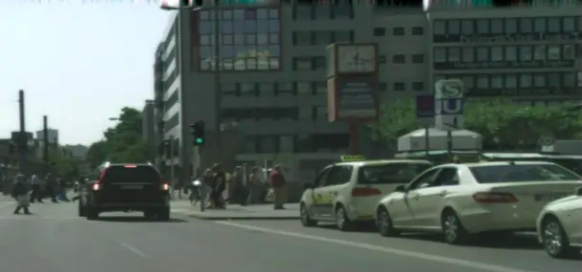
\includegraphics[width=0.60\textwidth]{images/figure0.png} % replace with your image file name
  \caption{Αυθεντική εικόνα}
  \label{figure 1}
\end{figure}

\begin{figure}[h!]
  \centering
  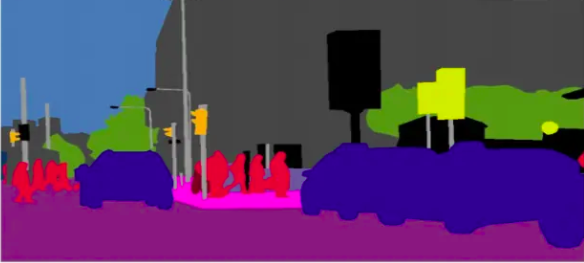
\includegraphics[width=0.6\textwidth]{images/figure1.png} % replace with your image file name
  \caption{Σημασιολογική κατάτμηση εικόνας}
  \label{figure 2}
\end{figure}

Όπως μπορούμε να δούμε στην εικόνα κάθε εικονοστοιχείο της αντιστοιχείζεται σε κάποια σημασιολογική κατηγορία. Μπορούμε να παρατηρήσουμε πως τα εικονοστοιχεία που αντιστοιχείζονται στην ίδια σημασιολογική κατηγορία είναι τα εικονοστοιχεία τα οποία αντιστοιχούν στο ίδιο "αντικείμενο" ή "σκηνικό" στοιχείο. \\

Μερικές σημαντικές μετρικές απόδοσης της σημασιολογικής κατάτμησης εικόνας είναι η Intersection over Union (IoU), όπως επίσης και η Pixel Accuracy (PA)~\cite{DBLP:journals/corr/abs-2001-05566}. Μερικά παραδείγματα σημείων αναφοράς (benchmarks) που χρησιμοποιούνται για την ποσοτικοποίηση της απόδοσης συγκεκριμένων αλγορίθμων που χρησιμοποιούν την τεχνική αυτή είναι τα Cityscapes~\cite{DBLP:journals/corr/CordtsORREBFRS16}, PASCAL VOC~\cite{Everingham2010} και ADE20K~\cite{8100027}. \\

\subsubsection{Κατάτμηση αντικειμένων}
Η ανίχνευση αντικειμένων αποτελεί διαδικασία κατά την οποία ο αλγόριθμος εντοπίζει και ταξινομεί τα "αντικείμενα" μιας εικόνας προσδιορίζοντας την θέση τους μέσω ορθογώνιων πλαισίων. Η σημασιολογική κατάτμηση εικόνας, όπως αναφέραμε παραπάνω προσδιορίζει την σημασιολογική κατηγορία κάθε εικονοστοιχείου μιας εικόνας, χωρίς όμως να διαχωρίζει μεταξύ διαφορετικών "αντικειμένων" της ίδιας κατηγορίας. Προχωρώντας ένα βήμα παραπέρα, η κατάτμηση αντικειμένων συνδυάζει αυτές τις 2 τεχνικές και παρέχει διαφορετικές ετικέτες για ξεχωριστές εμφανίσεις "αντικειμένων" που ανήκουν στην ίδια κατηγορία, αγνοώντας εντελώς τα "σκηνικά" στοιχεία~\cite{Hafiz_2020}. \\

\begin{figure}[h!]
  \centering
  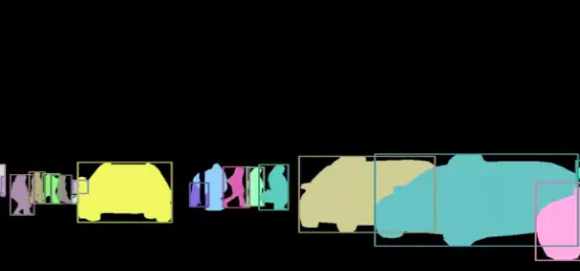
\includegraphics[width=0.6\textwidth]{images/figure2.png} % replace with your image file name
  \caption{Κατάτμηση παραδειγμάτων}
  \label{figure 3}
\end{figure}

Όπως μπορούμε να δούμε στην εικόνα παραπάνω το μοντέλο κατηγοριοποιεί μόνο τα εικονοστοιχεία τα οποία αντιστοιχούν σε "αντικείμενα", αδιαφορώντας για τα υπόλοιπα. Εύκολα μπορούμε να παρατηρήσουμε επίσης πως γίνετε διάκριση μεταξύ των "αντικειμένων" που ανήκουν στην ίδια κατηγορία.\\

Κάποιες σημαντικές μετρικές απόδοσης της κατάτμησης παραδείγματος είναι οι Average Precision (AP) και Mask Average Precision (Mask AP)~\cite{Hafiz_2020}. Μερικά παραδείγματα συνόλων αναφοράς που χρησιμοποιούνται για την ποσοστικοποίηση της απόδοσης συγκεκριμένων αλγορίθμων που χρησιμοποιούν την τεχνική αυτή είναι τα COCO~\cite{lin2015microsoftcococommonobjects}, Cityscapes~\cite{DBLP:journals/corr/CordtsORREBFRS16} και ADE20K~\cite{8100027}.

\subsubsection{Πανοπτική κατάτμηση εικόνας}

Η πανοπτική κατάτμηση εικόνας αποτελεί διαδικασία κατά την οποία γίνετε συνδυασμός της ανίχνευσης αντικειμένων και της σημασιολογικής κατάτμησης εικόνας. Συγκεκριμένα, στην πανοπτική κατάτμηση εικόνας πραγματοποιήτε κατηγοριοποίηση όλων των εικονοστοιχείων της εικόνας, ανεξάρτητα εάν τα εικονοστοιχεία αντιστοιχούν σε "αντικείμενα" ή "σκηνικά" στοιχεία και παράλληλα γίνετε διαχωρισμός μεταξύ των "αντικειμένων" που αντιστοιχούν στην ίδια σημασιολογική κατηγορία~\cite{elharrouss2021panopticsegmentationreview}.

\newpage

\begin{figure}[h!]
  \centering
  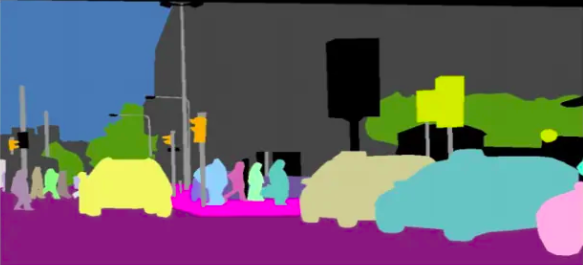
\includegraphics[width=0.6\textwidth]{images/figure3.png} % replace with your image file name
  \caption{Πανοπτική κατάτμηση εικόνας}
  \label{figure 4}
\end{figure}

Όπως μπορούμε να δούμε στην εικόνα παραπάνω το μοντέλο κατηγοριοποιεί όλα τα εικονοστοιχεία της εικόνας και ταυτόχρονα διαχωρίζει τα "αντικείμενα", τα οποία ανήκουν στην ίδια σημασιολογική κατηγορία. \\

Μερικές σημαντικές μετρικές της απόδοσης της πανοπτικής κατάτμησης εικόνας είναι η Panoptic Quality (PQ), η Segmentation Quality (SQ) και η Recognition Quality (RQ). Ωστόσο, γνωρίζουμε πως η πανοπτική κατάτμηση εικόνας αποτελεί συνδυασμό της σημασιολογικής κατάτμησης εικόνας και της κατάτμησης αντικειμένων υπάρχουν μετρικές που έχουν ώς σκοπό την ποσοτικοποίηση της απόδοσης των μοντέλων πανοπτικής κατάτμησης εικόνας στις 2 προηγούμενες εργασίες. Συγκεκριμένα για τα προαναφερθέντα υπάρχουν οι μετρικές απόδοσης Panoptic Quality Things (\(PQ_{th}\)) και Panoptic Quallity Stuff (\(PQ_{st}\))~\cite{elharrouss2021panopticsegmentationreview}. Μερικά παραδείγματα σημείων αναφοράς που χρησιμοποιούνται για την ποσοτικοποίηση της απόδοσης συγκεκριμένων αλγορίθμων που κάνουν χρήση της τεχνικής αυτής είναι τα COCO~\cite{lin2015microsoftcococommonobjects}, Cityscapes~\cite{DBLP:journals/corr/CordtsORREBFRS16} και ADE20K~\cite{8100027}.

\subsection{Σύνολα δεδομένων για πανοπτική κατάτμηση εικόνας}

Στην σύγχρονη εποχή η όραση υπολογιστών βασίζεται σχεδόν αποκλειστικά σε μεθόδους βαθιάς μάθησης. Γνωρίζουμε πως η λειτουργία τέτοιων μεθόδων απαιτεί ένα πολύ μεγάλο όγκο δεδομένων συνδυασμένο με τις κατάλληλες επισημειώσεις, ανάλογα πάντα με την εργασία που θέλουμε να πραγματοποιήσουμε. Για τον σκοπό αυτό έχουν δημιουργηθεί κατάλληλα σύνολα δεδομένων~\cite{article2} που έχουν ώς σκοπό την εκπαίδευση των μοντέλων σε συγκεκριμένες εργασίες όπως και για την ποσοτική αξιολόγιση της απόδοσης τους στις εργασίες αυτές. Μερικά απο αυτά παρουσιάζονται στην συνέχεια.

\subsubsection{Σύνολο δεδομένων COCO}

Το COCO (Common Objects in Context), αποτελεί σύνολο δεδομένων μεγάλου μεγέθους. Περιέχει συνολικά περισσότερες απο 330.000 εικόνες και είναι διαθέσιμο σε 2 κύριες εκδόσεις, την COCO 2014 και COCO 2017, οι οποίες περιλαμβάνουν σε μεγάλο βαθμό κοινές εικόνες αλλά με διαφορετικό διαχωρισμό σε σύνολα εκπαίδευσης και επικύρωσης. Κάθε μια απο αυτές τις εικόνες είναι επισημειωμένη με 80 κατηγορίες αντικειμένων και 5 ετικέτες που περιγράφουν την σκηνή. Το σύνολο δεδομένων χωρίζεται σε 2 κατηγορίες. Απο την μια έχουμε τις εικόνες, ενώ απο την άλλη τις αντίστοιχες επισημειώσεις. Οι εικόνες είναι  οργανωμένες ιεραρχικά σε φακέλους, με τον φάκελο που βρίσκεται στο υψηλότερο επίπεδο να περιέχει φακέλους για το σύνολο δεδομένων εκπαίδευσης (Train set), το σύνολο δεδομένων επικύρωσης (Validation set) και το σύνολο δεδομένων δοκιμής (Test set)~\cite{lin2015microsoftcococommonobjects},~\cite{shah2023coco}.  \\

Οι επισημειώσεις δίνονται σε JSON αρχεία, όπου κάθε αρχείο αντιστοιχεί σε μια εικόνα. Κάθε τέτοιο αρχείο περιέχει: \\

\begin{itemize}
    \item Το όνομα του αρχείου
    \item Το μέγεθος της εικόνας
    \item 5 ετικέτες που περιγράφουν την σκηνή
     \item Λίστα με τα αντικείμενα που υπάρχουν μέσα στην εικόνα (Για κάθε αντικείμενο περιέχεται η κατηγορία του, οι συντεταγμένες του ορθοφωνίου που το περιβάλλει, τα εικονοστοιχεία που αντιστοιχούν σε αυτό το αντικείμενο και τα σημεία κλειδιά του)
\end{itemize}

Το σύνολο δεδομένων COCO περιέχει επίσης την άδεια χρήσης, επισημειώσεις για τα "σκηνικά" στοιχεία, σε επίπεδο εικονοστοιχείου και υπερκατηγορίες αντικειμένων (Αποτελούν ευρύτερες κατηγορίες που περιλαμβάνουν πιο συγκεκριμένες υποκατηγορίες π.χ. dog \(\subset\) animal). Το σύνολο δεδομένων COCO μπορεί να χρησιμοποιηθεί σε εργασίες όπως η ανίχνευση αντικειμένων, η σημασιολογική κατάτμηση εικόνας, η πανοπτική κατάτμηση εικόνας κ.ο.κ.~\cite{shah2023coco}. \\

\noindent Παρακάτω δίνονται όλες οι κατηγορίες αντικειμένων που περιέχονται στο σύνολο δεδομένων COCO.

\begin{figure}[h!]
  \centering
  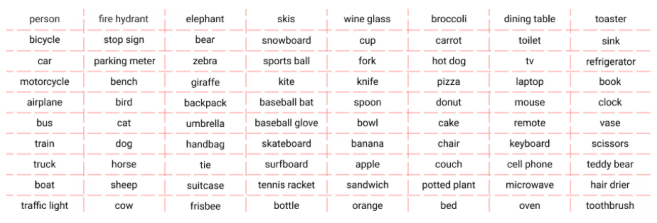
\includegraphics[width=0.9\textwidth]{images/coco.png} % replace with your image file name
  \caption{Κατηγορίες αντικειμένων συνόλου δεδομένων COCO}
  \label{figure 5}
\end{figure}

\noindent Είναι σημαντικό να αναφέρουμε πως το σύνολο δεδομένων COCO δεν περιέχει ισορροπημένο αριθμό αντικειμένων στις εικόνες κάτι που οδηγεί σε μεροληψία. Όπως αναφέραμε παραπάνω το σύνολο δεδομένων COCO έρχεται σε 2 κύριες εκδόσεις. Η COCO 2014 περιέχει 82.783 εικόνες στο σύνολο δεδομένων εκπαίδευσης, 40.504 εικόνες στο σύνολο δεδομένων επικύρωσης και 40.775 εικόνες στο σύνολο δεδομένων δοκιμής. Στα αντίστοιχα σύνολα το COCO 2017 έχει 118.287, 5.000 και 40.670 εικόνες~\cite{fan2021tao}. \\

Για την εργασία της πανοπτικής κατάτμησης εικόνας το σύνολο δεδομένων COCO περιέχει επίσης κατάλληλες επισημειώσεις για την συγκεκριμένη εργασία, όπου οι επισημειώσεις αυτές περιέχουν πληροφορία για 91 διαφορετικές κατηγορίες "σκηνικών" στοιχείων~\cite{lin2015microsoftcococommonobjects},~\cite{shah2023coco}. Η δομή του συνόλου δεδομένων δίνετε παρακάτω: \\

\begin{figure}[h!]
  \centering
  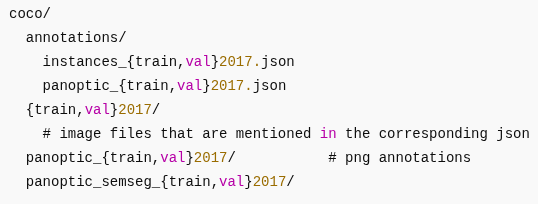
\includegraphics[width=0.7\textwidth]{images/coco_format.png} % replace with your image file name
  \caption{Δομή συνόλου δεδομένων COCO}
  \label{figure 6}
\end{figure}

\subsubsection{Σύνολο δεδομένων Cityscapes}

Η κατανόηση περίπλοκων αστικών σκηνών αποτελεί καθοριστικό παράγοντα για ένα ευρύ φάσμα εφαρμογών. Ωστόσο, δεν υπάρχουν πολλά σύνολα δεδομένων που να αποτυπόνουν επαρκώς την πολυπλοκότητα των σκηνών που παρουσιάζονται στον πραγματικό κόσμο. Λύση σε αυτό το πρόβλημα ήρθε να φέρει το σύνολο δεδομένων Cityscapes~\cite{DBLP:journals/corr/CordtsORREBFRS16}. \\


Το σύνολο δεδομένων Cityscapes δημιουργήθηκε μέσω επιλεγμένων καρέ (Frame), τα οποία εξήχθησαν απο στερεοσκοπικές ακολουθίες βίντεο που καταγράφηκαν απο κινούμενο όχημα στους δρόμους 50 διαφορετικών πόλεων, κυρίως της Γερμανίας. Απο τις εικόνες αυτές, οι 5.000 διαθέτουν υψηλής ποιότητας επισημειώσεις σε επίπεδο εικονοστοιχείου, ενώ οι υπόλοιπες 20.000 διαθέοτουν χαμηλότερης ποιότητας επισημειώσεις, έτσι ώστε να μπορούν να χρησιμοποιηθούν για την εκπαίδευση μοντέλων σε όχι πλήρως επισημειωμένα δεδομένα (Ασθενώς επιβλεπόμενη μάθηση). Απο τις 5.000 πλήρως επισημειωμένες εικόνες, οι 2.975 απο αυτές αποτελούν εικόνες του συνόλου δεδομένων εκπαίδευσης, οι 500 του συνόλου δεδομένων επικύρωσης και οι υπόλοιπες 1.525 του συνόλου δεδομένων δοκιμής. Οι πλήρως επισημειωμένες εικόνες εξήχθησαν χεροκίνητα απο 27 απο τις 50 πόλεις του συνόλου δεδομένων και συκγκεριμένα απο το 20ό καρέ αποσπασμάτων βίντεο διαρκείας 30 καρέ. Αντίθετα, οι υπόλοιπες ασθενώς επισημειωμένες εικόνες του συνόλου δεδομένων έχουν προέλευση απο τις υπόλοιπες 23 πόλεις και εξήχθησαν απο τα αντίστοιχα βίντεο εξάγωντας μια εικόνα ανά 20 δευτερόλεπτα λήψης βίντεο ή 20 μέτρα οδήγησης, ανάλογα με το πιο απο τα 2 συναίβενε πρώτο. Όπως μπορούμε να δούμε παρακάτω, το σύνολο δεδομένων Cityscapes περιλαμβάνει ετικέτες για συνολικά 30 "αντικείμενα", απο τα οποία μόνο τα 19 χρησιμοποιούνται στην επικύρωση των αποτελεσμάτων~\cite{DBLP:journals/corr/CordtsORREBFRS16}.\\

\begin{figure}[h!]
  \centering
  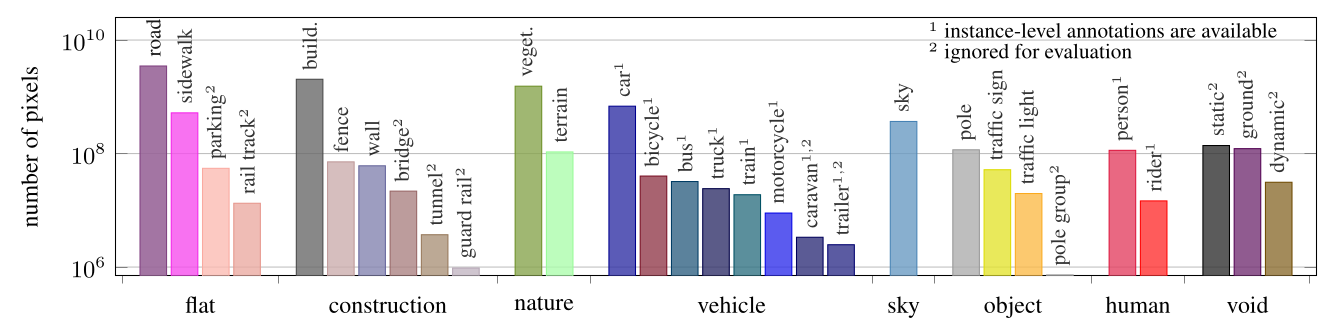
\includegraphics[width=0.9\textwidth]{images/cityscapes_objects.png} % replace with your image file name
  \caption{Αντικείμενα συνόλου δεδομένων Cityscapes}
  \label{figure 7}
\end{figure}

Το σύνολο δεδομένων περιλαμβάνει εικόνες καταγεγραμμένες κατά την διάρκεια της Άνοιξης, του Καλοκαιριού και του Φθινωπόρου και καλύπτει αρκετούς μήνες του έτους. Δεν περιλαμβάνει εικόνες με δυσμενείς καιρικές συνθήκες, όπως έντονη βροχόπτωση ή χιόνι επειδή οι συνθήκες αυτές απαιτούν την χρήση εξειδικευμένων τεχνικών και συνόλων δεδομένων. Όλες οι εικόνες είναι διαθέσιμες σε 8-bit (Low Dynamic Range) και 16-bit (High Dynamic Range), ώς πρός το βάθος χρώματος. Εκτός απο τις 8-bit, 16-bit εικόνες και τις αντίστοιχες επισημειώσεις, το σύνολο δεδομένων Cityscapes περιλαμβάνει πληροφορίες ώς πρός την εξωτερική θερμοκρασία, την διαδρομή που ακολούθησε το όχημα (GPS) και την οδομετρία του~\cite{DBLP:journals/corr/CordtsORREBFRS16}. \\

Το σύνολο δεδομένων Cityscapes μπορεί να χρησιμοποιηθεί για εργασίες όπως η σημασιολογική κατάτμηση εικόνας, η πανοπτική κατάτμηση εικόνας, η εκτίμηση βάθους κ.ο.κ. ~\cite{DBLP:journals/corr/CordtsORREBFRS16}, ~\cite{cheng2022maskedattentionmasktransformeruniversal}, ~\cite{taghavi2024swinmtlsharedarchitecturesimultaneous}.




\subsubsection{Σύνολο δεδομένων ADE20K}

Σε αντίθεση με την απλή κατανόηση του περιεχομένου μιας εικόνας (Image-level recognition), η κατανόηση σε επίπεδο εικονοστοιχείου (Pixel level scene understanding) απαιτεί σύνολα δεδομένων με πολύ πιο πυκνές επισημειώσεις και ένα ευρύ σύνολο "αντικειμένων". Ωστόσο, τα περισσότερα σύνολα δεδομένων παρουσιάζουν ένα περιορισμένο αριθμό "αντικειμένων" (π.χ. COCO~\cite{lin2015microsoftcococommonobjects}, Pascal VOC~\cite{Everingham2010}) και συχνά περιλαμβάνουν κατηγορίες που δεν είναι συνηφασμένες με τα πιο κοινά αντικείμενα που μπορούμε να συναντήσουμε στον πραγματικό κόσμο ή καλύπτουν μόνο ένα περιορισμένο φάσμα σκηνών (π.χ. Cityscapes~\cite{DBLP:journals/corr/CordtsORREBFRS16}). Εξαιρεση σε αυτό αποτελεί το σύνολο δεδομένων Pascal-Context~\cite{6909514}, όπως και η βάση δεδομένων Sun~\cite{5539970}, με το πρώτο να επικεντρώνεται κυρίως σε μόνο 20 κατηγορίες "αντικειμένων" ενώ το δεύτερο περιλαμβάνει επισημειώσεις "αντικειμένων" με υψηλό επίπεδο θορύβου. Η ανάγκη δημιουργίας ενός συνόλου δεδομένων, το οποίο να ανταποκρίνετε στα παραπάνω προβλήματα οδήγησε στη δημιουργία του συνόλου δεδομένων ADE20K~\cite{8100027}, ~\cite{zhou2018semanticunderstandingscenesade20k}. \\

Το ADE20K αποτελεί ένα εκτενώς επισημειωμένο σύνολο δεδομένων, με την έννοια πως για κάθε εικόνα παρέχονται λεπτομερείς ετικέτες που καλύπτουν "αντικείμενα", όπως και μέρη "αντικειμένων" ("υπο-αντικείμενα"). Αποτελείτε απο συνολικά 25.210 εικόνες ,όπου οι 20.210 απο αυτές αποτελούν εικόνες του συνόλου δεδομένων εκπαίδευσης,  οι 2.000 απο αυτές αποτελούν εικόνες του συνόλου δεδομένων επικύρωσης και οι υπόλοιπες 3.000 του συνόλου δεδομένων δοκιμής. Στις εικόνες υπάρχουν συνολικά 3169 επισημειώσεις απο τις οποίες οι 2693 απο αυτές αποτελούν τα "αντικείμενα" και "σκηνικά" στοιχεία και οι υπόλοιπες 476 αποτελούν μέρη μεγαλύτερων "αντικειμένων"¨. Στο σύνολο δεδομένων ADE20K υπάρχουν "υπο-αντικείμενα" μέχρι επιπέδου το πολύ 3. Παρακάτω δίνετε μια αναπαράσταση κάποιων απο τα "αντικείμενα" του συνόλου δεδομένων μαζί με τα αντίστοιχα "υπο-αντικείμενα" τους~\cite{8100027}, ~\cite{zhou2018semanticunderstandingscenesade20k}. \\

\begin{figure}[h!]
  \centering
  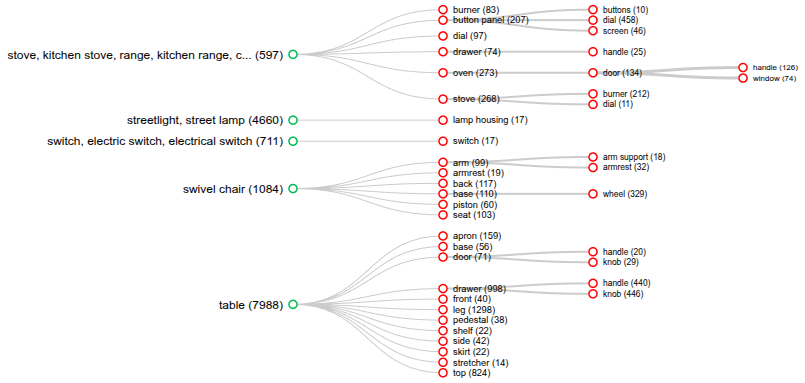
\includegraphics[width=0.8\textwidth]{images/ADE20K_objects.png} % replace with your image file name
  \caption{Αντικείμενα συνόλου δεδομένων ADE20K}
  \label{figure 8}
\end{figure}

Στο σύνολο δεδομένων ADE20K, το 76\% των "αντικειμένων" περιλαμβάνει "υπο-αντικείμενα" με μέσο όρο "υπο-αντικειμένων" που περιλαμβάνουν τα "αντικείμενα" αυτά ίσο με 3. Κατά μέσο όρο υπάρχουν 19.5 εμφανίσεις "αντικείμενων" και 10.5 διαφορετικές κατηγορίες "αντικείμενων" σε κάθε εικόνα. Ο ελάχιστος αριθμός "αντικειμένων" που υπάρχουν σε κάποια απο τις εικόνες του συνόλου δεδομένων είναι ίσος με 5 με κάποιες εικόνες να έχουν μέχρι και 273, χωρίς την συμπερίληψη των "υπο-αντικείμενων" σε αυτά. Συμπεριλαμβανομένων των "υπο-αντικειμένων" φτάνουμε μέχρι και 419~\cite{8100027}, ~\cite{zhou2018semanticunderstandingscenesade20k}. \\

Το σύνολο δεδομένων ADE20K μπορεί να χρησιμοποιηθεί για εργασίες όπως η σημασιολογική κατάτμηση εικόνας, η κατάτμηση αντικειμένων, η πανοπτική κατάτμηση εικόνας κ.ο.κ. ~\cite{8100027}, ~\cite{cheng2022maskedattentionmasktransformeruniversal}.


\subsection{Μετρικές απόδοσης πανοπτικής κατάτμησης εικόνας}

Οι μετρικές απόδοσης αποτελούν βασικό εργαλείο και διαδραματίζουν σημαντικό ρόλο για τη σύγκριση της αποτελεσματικότητας διαφορετικών μεθόδων σε διάφορες εργασίες. Η πανοπτική κατάτμηση εικόνας, όπως αναφέραμε και πρίν αποτελεί εργασία κατά την οποία συνδυάζεται η σημασιολογική κατάτμηση εικόνας και η κατάτμηση αντικειμένων. Αν και οι υπάρχουσες μετρικές απόδοσης της σημασιολογικής κατάτμησης εικόνας, όπως και της κατάτμησης αντικειμένων μπορούν σε κάποιο βαθμό να εφαρμοσθούν στην πανοπτική κατάτμηση εικόνας, δεν αρκούν απο μόνες τους. Συνήθως, για την συγκεκριμένη εργασία χρησιμοποιούνται μετρικές όπως η πανοπτική ποιότητα (Panoptic Quality - PQ), η ποιότητα κατάτμησης (Segmentation Quality - SQ) και η ποιότητα αναγνώρισης (Recognition Quality - RQ). Ωστόσο, μπορούν να χρησιμοποιηθούν και άλλες μετρικές για την σύγκριση της απόδοσης των μεθόδων αυτών όσον αφορά την σημασιολογική κατάτμηση και την κατάτμηση αντικειμένων, όπως ο περιορισμός των πιο πάνω μετρικών μόνο σε "αντικείμενα" (Things) ή μόνο σε "σκηνικά" στοιχεία (Stuff). Θα μπορούσαν επίσης να χρησιμοποιήσουμε μετρικές απόδοσης, όπως ο μέσος όρος ακρίβειας (Average Precision - AP) και η Intersection over Union (IoU)~\cite{elharrouss2021panopticsegmentationreview}. 

\subsubsection{Πίνακας σύγχυσης (Confusion matrix)}

Για να μπορέσουμε να ορίσουμε μερικές απο τις μετρικές απόδοσης που αναφέρθηκαν παραπάνω, χρειάζεται πρώτα να ορίσουμε τον πίνακα σύγχυσης. Ο πίνακας σύγχυσης αναπαριστά την ακρίβεια ενός μοντέλου ταξινόμησης. Παρουσιάζει τις τιμές των True positives (TP), των True negatives (TN), των False positives (FP) και των False negatives (FN). Ο πίνακας αυτός έχει μέγεθος NxN, όπου N είναι το πλήθος των κλάσεων ταξινόμησης και κάθε κελί του πίνακα αντιστοιχεί στο πλήθος των δειγμάτων που έχουν πραγματική τιμή ίδια με την πραγματική τιμή που αντιστοιχεί στο κελί και προβλεπόμενη τιμή ίδια με την προβλεπόμενη τιμή που αντιστοιχεί στο κελί. Στην ουσία συγκρίνεται η πραγματική ετικέτα με την ετικέτα η οποία προβλέφθηκε απο το μοντέλο. Για ένα δυαδικό πρόβλημα ταξινόμησης θα είχαμε τον παρακάτω πίνακα. 

\begin{figure}[h!]
  \centering
  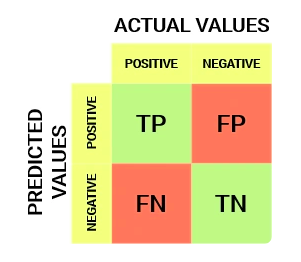
\includegraphics[width=0.4\textwidth]{images/conf_matrix.png} % replace with your image file name
  \caption{Μορφή πίνακα σύγχυσης για δυαδική ταξινόμηση}
  \label{figure 9}
\end{figure}

\noindent Στην περίπτωση αυτή το πρόβλημα είναι δυαδικό και ταξινομείτε σε 2 κλάσεις, την θετική (Positive) και την αρνητική (Negative). Όπως μπορούμε να δούμε και παραπάνω οι στήλες αναπαριστούν τις πραγματικές και οι γραμμές τις προβλεπόμενες τιμές. Παρακάτω δίνετε η ερμηνεία των TP, FP, FN και TN συκγκεκριμένα για δυαδικό πρόβλημα ταξινόμησης. \\

\noindent$\mathbf{TP: }$ Η προβλεπόμενη τιμή ανιστοιχεί με την πραγματική τιμή και η πραγματική τιμή ανήκει στην θετική κλάση (Positive). \\

\noindent$\mathbf{TΝ: }$ Η προβλεπόμενη τιμή ανιστοιχεί με την πραγματική τιμή και η πραγματική τιμή ανήκει στην αρνητική κλάση (Negative). \\

\noindent$\mathbf{FP: }$ Η προβλεπόμενη τιμή δεν ανιστοιχεί με την πραγματική τιμή. Η πραγματική τιμή ανήκει στην αρνητική κλάση αλλά το μοντέλο προέβλεψε πως ανήκει στην θετική. Το τιμή αυτή καλείτε και σφάλμα τύπου 1. \\

\noindent$\mathbf{FΝ: }$ Η προβλεπόμενη τιμή δεν ανιστοιχεί με την πραγματική τιμή. Η πραγματική τιμή ανήκει στην θετική κλάση αλλά το μοντέλο προέβλεψε πως ανήκει στην αρνητική. Η τιμή αυτή καλείτε και σφάλμα τύπου 2. \\

\noindent Στην περίπτωση που το πρόβλημα ταξινόμησης δεν είναι δυαδικό υπάρχουν διαφορές.  Συγκεκριμένα οι τιμές των TP, FP, FN και TN, υπολογίζονται για κάθε κατηγορία. Επομένως θα έχουμε \(TP_i, FP_i, FN_i, TN_i\), i = 1,...,N. Για κλάση i θα έχουμε: \\

\noindent $\mathbf{TP}_i:$ Ισούται με την τιμή του κελιού (i,i) στον πίνακα σύγχυσης. \\

\noindent $\mathbf{TN}_i:$ Ισούται με το άθροισμα $\sum_{p \neq i}^{N} \sum_{k \neq i}^{N} value(p,k)$, όπου value(i,j) η τιμή του πίνακα σύγχυσης στο κελί (i,j). \\

\noindent $\mathbf{FP}_i:$ Ισούται με το άθροισμα $\sum_{p \neq i}^{N} value(i,p)$, όπου value(i,j) η τιμή του πίνακα σύγχυσης στο κελί (i,j).\\

\noindent $\mathbf{FN}_i:$ Ισούται με το άθροισμα $\sum_{p \neq i}^{N} value(p,i)$, όπου value(i,j) η τιμή του πίνακα σύγχυσης στο κελί (i,j). \\




\noindent Αποφασίζουμε μέσω αυτής της μετρικής πως το μοντέλο ταξινόμησης είναι αποδοτικό εάν το πλήθος των True Positive και True Negative είναι μεγάλος σε σχέση με το συνολικό πλήθος των παρατηρήσεων~\cite{bhandari2025confusion}. 


\subsubsection{Intersection over Union (Intersection over Union - IoU)}

Αναφέρεται επίσης και ως δείκτης Jaccard. Πρόκειτε ουσιαστικά για ένα τρόπο ποσοτικοποίησης του ποσοστού επικάλυψης μεταξύ της μάσκας στόχου και της μάσκας πρόβλεψης. Συγκεκριμένα, η μετρική IoU μετρά το πλήθος των εικονοστοιχείων που είναι κοινά μεταξύ της μάσκας στόχου και της μάσκας πρόβλεψης, διαιρούμενο με τον συνολικό πλήθος των εικονοστοιχείων που υπάρχουν και στις δύο μάσκες μαζί~\cite{elharrouss2021panopticsegmentationreview}. \\

\begin{equation}
    IoU = \frac{target \cap prediction}{target \cup prediction}
\end{equation}
\\
Εύκολα μπορούμε να συμπεράνουμε πως \(0 \leq IoU \leq 1\).\\

\subsubsection{Μέσος Όρος Ακρίβειας (Average Precision - AP)}

Ο μέσος όρος ακριβείας αποτελεί την πιο ευρέως χρησιμοποιημένη μετρική απόδοσης στην κατάτμηση αντικειμένων~\cite{Kookna2022Segmentation}. Για την διατύπωση της μετρικής αυτής χρειάζεται πρώτα να ορίσουμε κάποιες άλλες μετρικές. Αρχικά, η ακρίβεια (Precision) για μια συγκεκριμένη κλάση μετρά το ποσοστό των προβλέψεων που ανήκουν στην κλάση αυτή και συμφωνούν με την πραγματική τιμή~\cite{Bex2021MulticlassMetrics}. Η ακρίβεια για μια κλάση k δίνεται απο την σχέση~\cite{grandini2020metricsmulticlassclassificationoverview}. \\

\begin{equation}
Precision_k = \frac{TP_k}{TP_k + FP_k}
\end{equation}\\

\noindent Στη συνέχεια θα ορίσουμε μια άλλη μετρική, την ανάκληση (Recall). Η ανάκληση για μια συγκεκριμένη κλάση μετρά το ποσοστό των "αντικειμένων" που ανήκουν στην κλάση αυτή και έχουν προβλεφθεί σωστά~\cite{Bex2021MulticlassMetrics}. Η ανάκληση για μια κλάση k δίνεται απο την σχέση~\cite{grandini2020metricsmulticlassclassificationoverview}.\\

\begin{equation}
Recall_k = \frac{TP_k}{TP_k + FN_k}
\end{equation}\\

Έπειτα ορίζουμε την καμπύλη ακριβείας-ανάκλησης (Precision-Recall curve). Η καμπύλη αυτή προκύπτει απεικονίζοντας τις τιμές ακριβείας και ανάκλησης του μοντέλου για μια συγκεκριμένη κλάση για όλες τις δυνατές τιμές του βαθμού εμπιστοσύνης. Ο μέσος όρος ακριβείας για κλάση k προκύπτει υπολογίζοντας το εμβαδόν κάτω απο την καμπύλη αυτή και δίνετε απο την σχέση.\\

\begin{equation}
AP_k = \int_{0}^{1} Precision(Recall) \, d(Recall)
\end{equation} \\

Ο μέσος όρος ακριβείας είναι άμεσα συνδεδεμένος με την τιμή του κατωφλίου της IoU που θα θέσουμε. Η τιμή του κατωφλίου επηρεάζει το πλήθος των προβλεπόμενων τμημάτων ίδιας κατηγορίας που αντιστοιχούν σε κάποιο πραγματικό τμήμα της εικόνας (Αντιστοίχιση τμημάτων)~\cite{Kirillov_2019_CVPR}, επιρεάζει δηλαδή τη σύνθεση των συνόλων \(TP_k, FP_k\) και \(FN_k\). Κατά συνέπεια, αυτό σημαίνει πως για διαφορετικές τιμές κατωφλίου λαμβάνουμε διαφορετική καμπύλη ακριβείας-ανάκλησης. \\

Για τον υπολογισμό της μετρικής mAP υπολογίζουμε την μέση τιμή των μέσων όρων ακριβείας (AP) για όλες τις κατηγορίες για κάποια τιμή του κατωφλίου της IoU. Αυτό δίνετε απο την σχέση. \\

\begin{equation}
mAP = \frac{1}{n} \sum_{k=1}^{n} AP_k
\end{equation}\\

Για τον υπολογισμόυ του τελικού mAP υπολογίζουμε την μέση τιμή των mAP για διαφορετικές τιμές του κατωφλίου της IoU. Ο τρόπος υπολογισμού της τελικής mAP διαφέρει ανάλογα με τον εκάστοτε διαγωνισμό ανίχνευσης αντικειμένων και συγκεκριμένα ώς πρός τις τιμές του κατωφλίου της IoU και των τιμών του βαθμού εμπιστοσύνης που επιλέγονται. Ενδεικτικά στον διαγωνισμό ανίχνευσης αντικειμένων COCO 2017~\cite{lin2015microsoftcococommonobjects} γίνετε χρήση συνολικά 10 διαφορετικών τιμών κατωφλίου, συγεκριμενα απο 0.5 εώς 0.95 με βήμα 0.05, καθώς και 101 τιμές βαθμών εμπιστοσύνης απο 0 μέχρι 1 με βημα 0.01~\cite{shah2022map}. \\



\subsubsection{Πανοπτική ποιότητα (Panoptic Quality - PQ)}

Η μετρική αυτή, σε αντίθεση με τις μετρικές που παρουσιάστηκαν προηγουμένως, αξιολογεί συνολικά την πανοπτική κατάτμηση εικόνας, λαμβάνοντας υπόψη τόσο τα "αντικείμενα" όσο και τα "σκηνικά" στοιχεία. Για την διατύπωση της μετρικής αυτής, απαιτείτε πρώτα ο ορισμός της έννοιας της αντιστοίχησης τμημάτων (Segment matching). Η αντιστοίχιση τμημάτων είναι η διαδικασία κατά την οποία αποφασίζεται ποιά απο τα προβλεπόμενα τμήματα που εξήγαγε το μοντέλο αντιστοιχούν σε ποιά πραγματικά τμήματα της εικόνας (Ground Truth). Για κάθε τμήμα τόσο για τα πραγματικά όσο και για τα προβλεπόμενα, κατασκευάζεται μια δυαδική μάσκα μεγέθους όσο και οι χωρικές διαστάσεις της εικόνας, όπου τα εικονοστοιχεία που αντιστοιχούν στο τμήμα παίρνουν την τιμή 1 ενώ τα υπόλοιπα την τιμή 0. Ένα προβλεπόμενο και ένα πραγματικό τμήμα, ίδιας κατηγορίας αντιστοιχούν μεταξύ τους εάν η μετρική IoU είναι μεγαλύτερη απο 0.5 (Κατώφλι). Η συνθήκη αυτή σε συνδυασμό με την ιδιότητα της μη επικάλυψης των τμημάτων που ισχύει στην πανοπτική κατάτμηση εικόνας εξασφαλίζει μοναδική αντιστοίχηση, δηλαδή μπορούμε να αντιστοιχίσουμε το πολύ ένα προβλεπόμενο για κάθε πραγματικό τμήμα της εικόνας. Η απόδειξη βρίσκεται στο ~\cite{Kirillov_2019_CVPR}.\\

Για χαμηλότερες τιμές του κατωφλίου της IoU απαιτούνται διαφορετικές τεχνικές αντιστοίχησης. Ωστόσο, στην πράξη ταιριάσματα με \(IoU \leq 0.5 \) είναι σπάνια, επομένως χαμηλότερα κατώφλια είναι περιττά. \\

Για τον υπολογισμό της πανοπτικής ποιότητας, υπλογίζουμε πρώτα την πανοπτική ποιότητα για κάθε κατηγορία ξεχωριστά και στη συνέχεια υπολογίζουμε τον μέσο όρο. Αυτό καθιστά την πανοπτική ποιότητα ανεπηρέαστη απο ανισσοροπία μεταξύ των κατηγοριών. Για κάθε κατηγορία, η μοναδική αντιστοίχιση που προέκυψε χωρίζει τα πραγματικά και προβλεπόμενα τμήματα σε 3 σύνολα, το True Positives (TP), το False Positives (FP) και το False Negatives (FN), όπου το πρώτο σύνολο συμβολίζει τα ζευγάρια πραγματικών και προβλεπόμενων τμημάτων που αντιστοιχίστηκαν μεταξύ τους, το δεύτερο σύνολο συμβολίζει τα προβλεπόμενα τμήματα που δεν αντιστοιχίστηκαν με κανένα πραγματικό τμήμα και το τρίτο σύνολο τα πραγματικά τμήματα που δεν αντιστοιχήστηκαν με κανένα προβλεπόμενο τμήμα. Αυτό αποτυπώνεται και στο παρακάτω παράδειγμα, όπου φαίνετε πώς τα τμήματα της κατηγορίας "person" διαχωρίζονται στα σύνολα True Positive, False Negative και False Positive~\cite{Kirillov_2019_CVPR}. \\

\begin{figure}[h!]
  \centering
  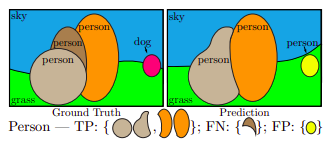
\includegraphics[width=0.6\textwidth]{images/PS_GT.png} % replace with your image file name
  \caption{Παράδειγμα υπολογισμού συνόλων TP, FP και FN για την κατηγορία "person"}
  \label{figure 10}
\end{figure}

\noindent Όπως μπορούμε να δούμε παραπάνω, το πραγματικό τμήμα κατηγορίας "person" χρώματος καφέ δεν αντιστοιχήστηκε με κάποιο προβλεπόμενο τμήμα, επομένως προστίθεται στο σύνολο FN. Το προβλεπόμενο τμήμα κατηγορίας "person" χρώματος κίτρινο δεν αντιστοιχήστηκε με κάποιο πραγματικό τμήμα, επομένως προστίθεται στο σύνολο FP. Τέλος, τα  προβλεπόμενα τμήματα κατηγορία "person" χρώματων γκρί και πορτοκαλί, αντιστοιχήστηκαν με 2 διαφορετικά πραγματικά τμήματα, επομένως τα ζευγάρια αυτά προστίθενται στο σύνολο TP. \\

\noindent Η πανοπτική ποιότητα μιας συγκεκριμένης κατηγορίας υπολογίζεται μέσω της παρακάτω σχέσης. \\

\begin{equation}
PQ = \frac{\sum_{(p, g) \in TP} \mathrm{IoU}(p, g)}{|TP| + \tfrac{1}{2}|FP| + \tfrac{1}{2}|FN|}
\end{equation}\\

Παρατηρώντας προσεκτικά, βλέπουμε πως η τιμή \(\frac{\sum_{(p, g) \in TP} \mathrm{IoU}(p, g)}{|TP| }\), είναι απλώς ο μέσος όρος της IoU για τα ταιριασμένα τμήματα, ενώ οι όροι \(\tfrac{1}{2}|FP| + \tfrac{1}{2}|FN|\) προσθίτενται στον παρονομαστή για να επιβάλλουν ποινή στα τμήματα που δεν έχουν ταίριασμα. Παρατηρούμε πως όλα τα τμήματα μετράνε το ίδιο στον υπολογισμό της πανοπτικής ποιότητας ανεξάρτητα απο των αριθμό των εικονοστοιχείων που καταλαμβάνουν στην εικόνα. Επίσης, μπορούμε να παρατηρήσουμε πως πολλαπλασιάζοντας και διαιρώντας την μετρική με |TP|, η πανοπτική ποιότητα μπορεί να γραφεί ώς ο πολλαπλασιαμός των μετρικών της ποιότητας κατάτμησης (Segmentation Quality - SQ) και ποιότητας αναγνώρισης (Recognition Quality - RQ)~\cite{Kirillov_2019_CVPR}. \\

\begin{equation}
PQ = \underbrace{\frac{\sum_{(p,g)\in TP} \mathrm{IoU}(p,g)}{|TP|}}_{\text{segmentation quality (SQ)}} \times \underbrace{\frac{|TP|}{|TP| + \tfrac{1}{2}|FP| + \tfrac{1}{2}|FN|}}_{\text{recognition quality (RQ)}}
\end{equation} \\

\noindent Επομένως, ισχύει πως PQ = SQ x RQ. \\

\noindent Μπορούμε να παρατηρήσουμε πως η ποιότητα αναγνώρισης αντιστοιχεί στο μισό της τιμής του γνωστού F1-score, το οποίο χρησιμοποιείτε ως μετρική ποιότητας της ανίχνευσης αντικειμένων~\cite{elharrouss2021panopticsegmentationreview}. Η ποιότητα κατάτμησης απο την άλλη αποτελεί την μέση τιμή των IoU των ταιριασμένων τμημάτων μιας συγκεκριμένης κατηγορίας. Προκειμένου να υπολογίσουμε την συνολική πανοπτική ποιότητα υπολογίζουμε τον μέσο όρο της πανοπτικής ποιότητας κατά μήκος όλων των κατηγοριών~\cite{Kirillov_2019_CVPR}.  \\

\begin{equation}
PQ_{\text{overall}} = \frac{1}{C} \sum_{c=1}^{C} PQ_c
\end{equation} \\

\noindent Περιορίζοντας τις μετρικές PQ, SQ και RQ μόνο στα "αντικείμενα", λαμβάνουμε τις μετρικές απόδοσης \(PQ_{th}, SQ_{th}\) και \(RQ_{th}\). Αντίστοιχα περιορίζοντας στα "σκηνικά" στοιχεία λαμβάνουμε τις μετρικές \(PQ_{st}, SQ_{st}\) και \(RQ_{st}\). Οι μετρικές αυτές χρησιμοποιούνται για να αποτυπώσουν την ποιότητα στην σημασιολογική κατάτμηση εικόνας και την κατάτμηση αντικειμένων~\cite{elharrouss2021panopticsegmentationreview}.\\

\noindent Στη συνέχεια θα αναλύσουμε πως αντιμετωπίζονται οι κενές ετικέτες (void labels) και οι ετικέτες ομάδας (group labels). Οι κενές ετικέτες δηλώνουν, σε επίπεδο εικονοστοιχείου, περιοχές της εικόνας που δεν αντιστοιχούν σε κάποιο "αντικείμενο" ή "σκηνικό" στοιχείο. Στις εικόνες αναφοράς (Ground Truth), αυτό οφείλετε είτε στο ότι τα εικονοστοιχεία αυτών των τμημάτων είναι πολύ δύσκολο να κατηγοριοποιηθούν με σιγουριά, είτε τα εικονοστοιχεία αυτά δεν ανήκουν σε καμιά απο τις κατηγορίες "αντικειμένων" ή "σκηνικών" στοιχείων που ορίζονται στο πρόβλημα. Εικονοστοιχεία τα οποία αντιστοιχούν σε κενή ετικέτα στις εικόνες αναφοράς, δεν λαμβάνονται υπόψη στην αξιολόγηση. Συγκεκριμένα, στην διαδικασία της αντιστοίχισης μεταξύ των προβλεπόμενων και πραγματικών τμημάτων, όλα τα εικονοστοιχεία στο προβλεπόμενο τμήμα τα οποία είναι επισημειωμένα ώς κενά στην εικόνα αναφοράς αφαιρούνται απο τo πρoβλεπόμενο τμήμα και δεν λαβμάνονται υπόψη στον υπολογισμό της IoU. Επίσης, όσα προβλεπόμενα τμήματα δεν ταίριαξαν με κανένα πραγματικό τμήμα και περιλαμβάνουν ποσοστό εικονοστοιχείων τα οποία αντιστοιχούν σε κενές ετικέτες στις εικόνες αναφοράς μεγαλύτερο απο την τιμή του κατωφλίου της IoU, αφαιρούνται και δεν προστίθενται στο σύνολο False Positive (FP).  Ακόμη, η τελική πρόβλεψη είναι δυνατό να περιέχει εικονοστοιχεία με κενές ετικέτες, δηλαδή το μοντέλο να μην προέβλεψε κάποια κατηγορία "αντικειμένου" ή "σκηνικού" στοιχείου για αυτά. Τα εικονοστοιχεία αυτά δεν λαμβάνονται υπόψη στην αξιολόγηση. Όσον αφορά τώρα τις ετικέτες ομάδας, χρησιμοποιούνται σε περιπτώσεις όπου υπάρχει πλήθος όμοιων "αντικειμένων" συγκεντρωμένο και είναι δύσκολος ο διαχωρισμός τους σε ξεχωριστά "αντικείμενα". Στον υπολογισμό της πανοπτικής ποιότητας, κατά την διαδικασία της αντιστοίχισης δεν λαμβάνονται υπόψη τα τμήματα τα οποία έχουν ετικέτα ομάδας. Επιπρόσθετα, για τα προβλεπόμενα τμήματα τα οποία δεν ταίριαξαν με κανένα πραγματικό τμήμα και περιλαμβάνουν ποσοστό εικονοστοιχείων τα οποία αντιστοιχούν σε ετικέτα ομάδας στις εικόνες αναφοράς, μεγαλυτερο απο την τιμή του κατωφλίου της IoU, αφαιρούνται και δεν προστίθενται στο σύνολο False Positive~\cite{Kirillov_2019_CVPR}.
\newpage

\section{Θεωρητικό υπόβαθρο}

\subsection{Ο νευρώνας}

Η έρευνα σχετικά με τα τεχνητά νευρωνικά δίκτυα είναι εμπνευσμένη απο την δομή και λειτουργία του εγκεφάλου. Βασικό δομικό του στοιχείο είναι  οι νευρώνες. Κίνητρο για την μελέτη του νευρώνα είναι η ανακάλυψη ενός μοντέλου το οποίο θα προσομοιώνει την λειτουργία και τις δυνατότητες του εγκεφάλου. Ωστόσο, τα τεχνητά νευρωνικά δίκτυα χρησιμοποιούν πολύ απλοποιημένα μοντέλα νευρώνων, τέτοια ώστε να διατηρούν μόνο τα πολύ αδρά χαρακτηριστικά των λεπτομερών μοντέλων που χρησιμοποιούνται στη νευρολογία. Οι λεπτομέρειες πιστεύεται πως δεν παίζουν ιδιαίτερη σημασία στην κατανόηση της ευφυούς συμπεριφοράς των βιολογικών νευρωνικών συστημάτων. Ακόμα και αυτά τα απλά μοντέλα νευρώνων μπορούν να δημιουργήσουν ιδιαιτέρως ενδιαφέροντα δίκτυα, αρκεί να πληρούν 2 βασικά χαρακτηριστικά.

\begin{itemize}
    \item Οι νευρώνες πρέπει να έχουν ρυθμιζόμενες παραμέτρους ώστε να διευκολύνεται η διαδικασία της μάθησης (Πλαστικότητα των νευρώνων).
    \item Το δίκτυο πρέπει να αποτελείτε απο μεγάλο πλήθος νευρώνων ώστε να επιτυγχάνεται παραλληλισμός της επεξεργασίας και κατανομή της πληροφορίας.
\end{itemize}

Ο νευρώνας αποτελεί ένα μεγάλο σε μέγεθος κύτταρο το οποίο αποτελείτε από τον πυρήνα, τους δενδρίτες, τον άξονα και τις συνάψεις που συνδέουν τις διακλαδώσεις του άξονα με τους δενδρίτες άλλων νευρώνων~\cite{zhang2019basicneuralunitsbrain}. \\

\begin{figure}[h!]
  \centering
  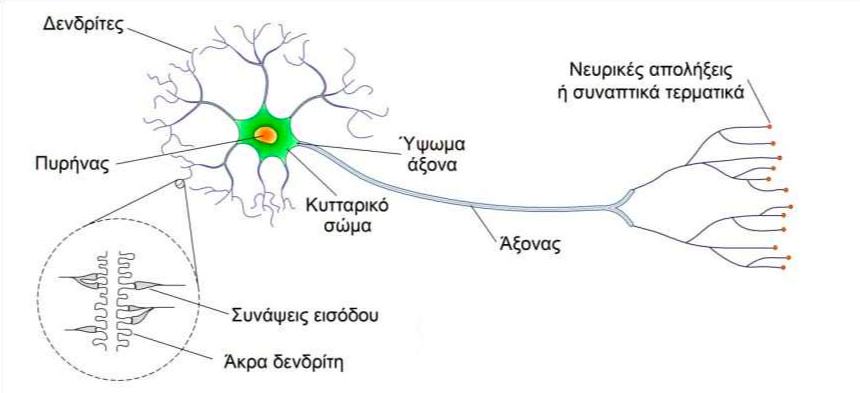
\includegraphics[width=0.6\textwidth]{images/neuron.png} % replace with your image file name
  \caption{Δομή νευρώνα}
  \label{figure 9}
\end{figure}

Λειτουργικά, τα τμήματα του νευρώνα παίζουν διαφορετικούς ρόλους. Οι δενδρίτες είναι οι πύλες του νευρώνα και δέχονται ηλεκτρικά σήματα από άλλους νευρώνες. Ο άξονας είναι η πύλη εξόδου του νευρώνα και στέλνει σήματα πρός άλλους νευρώνες υπό μορφή ηλεκτρικών παλμών σταθερού πλάτους αλλά μεταβλητής συχνότητας. Τέλος, οι συνάψεις είναι τα σημεία ένωσης μεταξύ των διακλαδώσεων του άξονα ενός νευρώνα και των δενδριτών από άλλους νευρώνες. Το πλάτος της σύναψης, η απόσταση της απο τον δενδρίτη και η πυκνότητα του ηλεκτροχημικού υλικού επηρεάζουν την ευκολία με την οποία η ηλεκτρική δραστηριότητα διαδίδεται απο τον άξονα στον δενδρίτη. Το ποσοστό της ηλεκτρικής δραστηριότητας που μεταδίδεται τελικά στον δενδρίτη ονομάζεται συναπτικό βάρος. Οι συνάψεις χωρίζονται σε ενισχυτικές (Exitatory) και ανασταλτικές (Inhibitory), ανάλογα με το αν το φορτίο που ελκύεται απο τη σύναψη διεγείρει τον νευρώνα για να παράγει παλμούς ή αντίθετα τον αναστέλλει εμποδίζοντας τον. \\

Στους βιολογικούς νευρώνες, οι φορείς των πληροφοριών είναι οι ηλεκτρικοί παλμοί, που ταξιδεύουν στον άξονα κάθε νευρώνα και μέσω των συνάψεων διαδίδονται στους δενδρίτες των νευρώνων. Κάθε νευρώνας συλλέγει όλο το ηλεκτρικό φορτίο που δέχεται απο κάθε σύναψη στους δενδρίτες του, σταθμόζοντας το εισερχόμενο φορτίο με το αντίστοιχο συναπτικό βάρος. Έτσι, όσο πιο ισχυρή είναι η συναπτική ζεύξη τόσο πιο πολύ συμμετέχει το συγκεκριμένο φορτίο εισόδου στο συνολικό άθροισμα. Άν το άθροισμα αυτό υπερβαίνει κάποιο κατώφλι (Threshhold), ο άξονας του νευρώνα αρχίζει να παράγει ηλεκτρικούς παλμούς με μεγάλη συχνότητα, άν όμως δεν υπερβαίνει το συγκεκριμένο όριο, τότε ο νευρώνας παράγει πολύ αραιά παλμούς σε τυχαίες χρονικές στιγμές (Αδρανής νευρώνας). Τελικά οι παλμοί που παράγονται ταξιδεύουν κατά μήκος του άξονα και τροφοδοτούν τους άλλους νευρώνες με τους οποίους συνδέεται ο νευρώνας που παρείγαγε τον παλμό~\cite{zhang2019basicneuralunitsbrain}.

\subsection{Το μοντέλο McCulloch-Pitts}

Το μοντέλο McCulloch-Pitts αποτελεί το πρώτο μαθηματικό μοντέλο τεχνητού νευρώνα. Προτάθηκε το 1943 από τους Warren McCulloch και Walter Pitts και σχεδιάστηκε για να προσομοιώσει τη λειτουργία ενός βιολογικού νευρώνα, χρησιμοποιώντας λογικές πράξεις. Η κατάσταση του νευρώνα περιγράφεται απο ένα δυαδικό αριθμό y.

\begin{itemize}
    \item y = 0, ο νευρώνας είναι αδρανής
    \item y = 1, ο νευρώνας πυροδοτεί παλμούς (Δεν είναι αδρανής)
\end{itemize}

Οι συνάψεις περιγράφονται απο τα συναπτικά βάρη \(w_i \in \mathbb{R}\), i = 1,...,n. Έστω πως \(x_1\),\(x_2\),...,\(x_n\) είναι οι εισόδοι του νευρώνα, ελέγχουμε εάν το άθροισμα \(x_1w_1\)+...+\(x_nw_n\) του φορτίου που δέχεται ο νευρώνας είναι μεγαλύτερο απο κάποιο κατώφλι θ. Εάν ισχύει τότε ο νευρώνας πυροδοτεί παλμούς. Διαφορετικά ο νευρώνας παραμένει αδρανής. Αυτό είναι ισοδύναμο με το εάν εάν η ποσότητα


\begin{equation}
\large
u = \sum_{i=1}^{n} w_i x_i - \theta
\end{equation}

\noindent είναι μεγαλύτερη ή μικρότερη από το μηδέν, οπότε η έξοδος του νευρώνα ισούται με

\begin{equation}
\large
y = f(u) =
\begin{cases}
1 & \text{εάν } u > 0 \\
0 & \text{εάν } u \leq 0
\end{cases}
\end{equation}

Η συνάρτηση u καλείτε διέγερση του νευρώνα και η f(\(\cdot\)) συνάρτηση ενεργοποίησης. Στο μοντέλο McCulloch-Pitts η συνάρτηση ενεργοποίησης είναι η βηματική συνάρτηση 0/1. Η διέγερση u μπορεί να γραφεί επίσης και με την παρακάτω συνοπτική μορφή.

\begin{equation}
\large
u = \bar{w}^\top \bar{x} - \theta
\end{equation}

,όπου \(\bar{w}\) = \([w_1,...,w_n]^\top\) είναι το διάνυσμα των συναπτικών βαρών και \(\bar{x}\) = \([x_1,...,x_n]^\top\) είναι το διάνυσμα εισόδου. Το κατώφλι θ είναι ενας πραγματικός αριθμός όπως και τα \(w_1,...,w_n\). Κατ'αυτή την έννοια μπορούμε να απλοποιήσουμε την εξίσωση θέτοντας \(w_0\) = -\(\theta\), το οποίο θα ονομάζεται πόλωση και θα είναι συνδεδεμένο με μια σταθερή είσοδο \(x_0\) = 1. Επομένως, τώρα έχουμε 

\begin{equation}
\large
u = \sum_{i=0}^{n} w_i x_i 
\end{equation}

\noindent Παρακάτω δίνετε η σχηματική αναπαράσταση του μοντέλου McCulloch-Pitts.

\begin{figure}[h!]
  \centering
  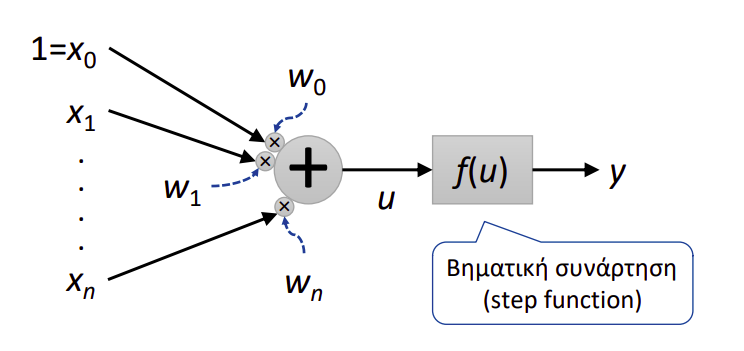
\includegraphics[width=0.7\textwidth]{images/McCulloch-Pitts.png} % replace with your image file name
  \caption{Μοντέλο McCulloch και Pitts του νευρώνα}
  \label{figure 10}
\end{figure}

\subsubsection{Εναλλακτικές συναρτήσεις ενεργοποίησης} 

Υπάρχουν πολλές διαφορετικές μοντελοποιήσεις του νευρώνα που αποκλίνουν απο το μοντέλο McCulloch-Pitts. Η πιο σημαντική διαφορά εντοπίζεται στη μορφή της μη γραμμικής συνάρτησης f(\(\cdot\)) που χρησιμοποιείτε στην έξοδο. Παρακάτω δίνετε η σχηματική αναπαράσταση μοντελοποίησης του νευρώνα που περιγράψαμε παραπάνω. \\

\begin{figure}[h!]
  \centering
  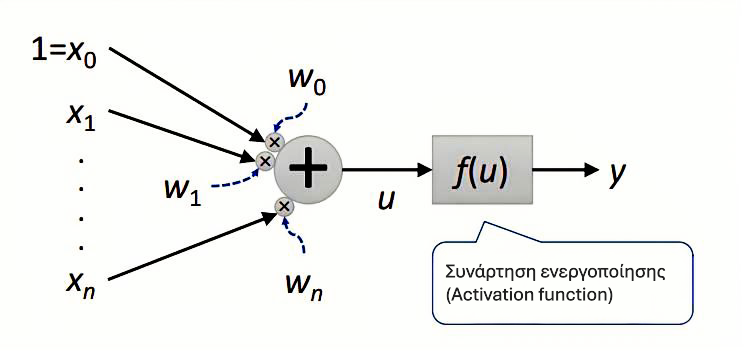
\includegraphics[width=0.7\textwidth]{images/neuron_modeling.png} % replace with your image file name
  \caption{Σχηματική αναπαράσταση του νευρώνα}
  \label{figure 11}
\end{figure} 

\noindent Η συνάρτηση ενεργοποίησης μπορεί να πάρει εναλλακτικά μεταξύ άλλων τις παρακάτω μορφές.\\

\paragraph{Βηματική συνάρτηση -1/1 (Step function -1/1)\\[0.5cm]}

Η βηματική συνάρτηση -1/1, όπως και η βηματική συνάρτηση 0/1 αποτελούν ειδικές περιπτώσεις μιας οικεγένειας συναρτήσεων που ονομάζονται βηματικές συναρτήσεις 2 επιπέδων (Binary step functions). Συγκεκριμένα, οι συναρτήσεις αυτού του τύπου, παραμένουν ανενεργές για τιμές μικρότερες ή ίσες με το κατώφλι (Στην περίπτωση μας το κατώφλι είναι ίσο με 0) και ενεργοποιούνται για τιμές μεγαλύτερες απο αυτό. Η βηματική συνάρτηση -1/1 δίνεται απο την σχέση \\

\begin{equation}
\large
y = f(u) =
\begin{cases}
1 & \text{εάν } u > 0 \\
-1 & \text{εάν } u \leq 0
\end{cases}
\end{equation} \\

Το σημαντικότερο μειονέκτημα των συναρτήσεων αυτής της οικογένειας είναι ότι σε όλα τα σημεία τους έχουν είτε μηδενική κλίση είτε δεν είναι διαφορίσιμες (Συγκεκριμένα στο σημείο του κατωφλίου). Αυτό το μειονέκτημα σηνιστά σημαντικό εμπόδιο για την εκπαίδευση νευρωνικών δικτύων πολλών στρωμάτων. Για αυτό το λόγο, συναρτήσεις αυτής της μορφής χρησιμοποιούνται αποκλειστικά σε νευρωνικά δίκτυα με ένα μόνο στρώμα~\cite{Navlani2022Activation}. Η γραφική μορφή της βηματικής συνάρτησης -1/1 δίνετε παρακάτω.

\begin{figure}[h!]
  \centering
  \includegraphics[width=0.5\textwidth]{images/Binary_step.png} % replace with your image file name
  \caption{Γραφική μορφή βηματικής συνάρτησης -1/1}
  \label{figure 11}
\end{figure}

\paragraph{Σιγμοειδής συνάρτηση (Sigmoid function)\\[0.5cm]} 

Αναφέρεται επίσης και ως λογιστική συνάρτηση. Αποτελεί μη γραμμική συνάρτηση, η οποία χρησιμοποιείτε συνήθως σε νευρωνικά δίκτυα μιας κατεύθυνσης (Feedforward neural networks). Είναι φραγμένη και διαφορίσιμη με θετική παράγωγο για όλα τα σημεία του πεδίοιυ ορισμού της, είναι δηλαδή γνησίως αύξουσα. Έχει πεδίο ορισμού το \(\mathbb{R}\) και σύνολο τιμών το (0,1). Δίνετε απο την σχέση \\

\begin{equation}
f(u) = \frac{1}{1 + e^{-u}}
\end{equation}  \\

Η σιγμοειδής συνάρτηση εμφανίζεται συνήθως στα στρώματα εξόδου των δικτύων βαθιάς μάθησης όταν θέλουμε η έξοδος να είναι υπό μορφή πιθανότητας. Παρά τα πλεονεκτήματα της όπως η εύκολη κατανόηση της και η καλή απόδοση της σε δίκτυα μικρού βάθους έχει κάποια σημαντικά μειονεκτήματα. Μερικά απο αυτά τα μειονεκτήματα περιλαμβάνουν την απότομη εξασθένιση των κλίσεων (Gradient) καθώς μεταφέρεται απο τα βαθύτερα πρός τα αρχικά στρώματα κατά την διαδικασία της οπισθοδρόμισης (Backpropagation), τον κορεσμό της λόγω των πολύ μικρών κλίσεων για μικρές αρνητικές και μεγάλες θετικές τιμές της εισόδου της συνάρτησης ενεργοποίησης καθώς και στο γεγονός πως η σιγμοδειδής συνάρτηση δεν είναι κεντραρισμένη στο 0, κάτι που μπορεί να οδηγήσει τις ανανεώσεις των βαρών να πραγματοποιούνται σε διαφορετικές κατευθύνσεις. Τα μειονεκτήματα αυτά μπορεί να δημιουργήσουν προβλήματα κατά την διαδικασία της εκπαίδευσης του μοντέλου όπως αργή σύγκλιση και αστάθεια κατά την διάρκεια της εκπαίδευσης~\cite{nwankpa2018activationfunctionscomparisontrends}. Η γραφική μορφή της σιγμοειδής συνάρτησης δίνετε παρακατω. \\

\begin{figure}[h!]
  \centering
  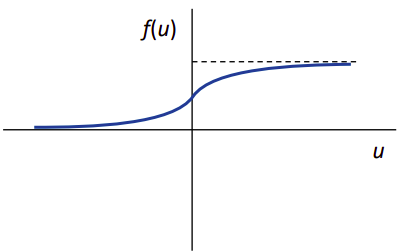
\includegraphics[width=0.5\textwidth]{images/Sigmoid.png} % replace with your image file name
  \caption{Γραφική μορφή σιγμοειδής συνάρτησης}
  \label{figure 12}
\end{figure}

\paragraph{Υπερβολική εφαπτομένη (Hyperbolic tangent)\\[0.5cm]}

Για την αντιμετώπιση ορισμένων προβλημάτων που εμφανίζονται χρησιμοποιώντας την σιγμοειδή συνάρτηση ως συνάρτησης ενεργοποίησης, προτάθηκε η χρήση της υπερβολικής εφαπτομένης. Η υπερβολική εφαπτομένη αποτελεί συνάρτηση κεντραρισμένη στο 0, με πεδίο ορισμού το \(\mathbb{R}\) και σύνολο τιμών το (-1,1). Αποτελεί προτιμόμενη επιλογή σε σχέση με την σιγμοειδή συνάρτηση, καθώς διευκολύνει την εκπαίδευση νευρωνικων δικτύων πολλών στρωμάτων περιορίζοντας φαινόμενα που μπορεί να εμφανιστούν χρησιμοποιώντας ώς συνάρτηση ενεργοποίησης την σιγμοειδή συνάρτηση. Ωστόσο, η υπερβολική εφαπτομένη δεν επιλύει το πρόβλημα της εξασθένισης των κλίσεων που εμφανίζεται χρησιμοποιώντας την σιγμοειδή συνάρτηση. Το βασικό της πλεονέκτημα είναι πως παράγει έξοδο κεντραρισμένη στο 0, διευκολύνοντας έτσι την διαδικασία της εκπαίδευσης του μοντέλου. Δίνεται απο την σχέση \\

\begin{equation}
f(u) = tanh(u) = \frac{1 - e^{-u}}{1 + e^{-u}}
\end{equation}\\

Είναι σημαντικό να αναφέρουμε πως η υπερβολική εφαπτομένη έχει κλίση ίση με 1, μόνο όταν η τιμή της εισόδου είναι ίση με 0. Αυτό έχει σαν αποτέλεσμα η συνάρτηση να δημιουργεί νεκρούς νευρώνες. Νεκρό νευρώνα ονομάζουμε μια κατάσταση κατά την οποία ο νευρώνας δεν χρησιμοποιείτε σχεδόν καθόλου κατά την διάρκεια της εκπαίδευσης ώς αποτέλεσμα των σχεδόν μηδενκών κλίσεων. Λύση στο πρόβλημα αυτό ήρθε να δώσει η συνάρτηση ενεργοποίησης ράμπας (ReLU activation function)~\cite{nwankpa2018activationfunctionscomparisontrends}. Η γραφική μορφή της συνάρτησης υπερβολικής εφαπτομένης δίνετε παρακάτω.\\

\begin{figure}[h!]
  \centering
  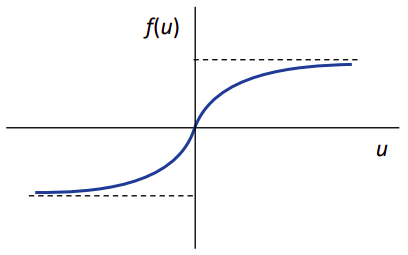
\includegraphics[width=0.5\textwidth]{images/Tanh.png} % replace with your image file name
  \caption{Γραφική μορφή υπερβολικής εφαπτομένης}
  \label{figure 13}
\end{figure} 

\paragraph{Συνάρτηση ράμπας (ReLU)\\[0.5cm]}

Η συνάρτηση αυτή αποτελεί την πιο ευρέως χρησιμοποιημένη συνάρτηση ενεργοποίησης στα μοντέλα βαθιάς μάθησης με κορυφαία αποτελέσματα μέχρι και σήμερα. Η συνάρτηση ράμπας επιτρέπει γρήγορη εκπαίδευση του μοντέλου και αποτελεί την πιο επιτυχημένη συνάρτηση ενεργοποίησης μέχρι και σήμερα. Έχει παρουσιάσει καλύτερη απόδοση από τη σιγμοειδή και την υπερβολική εφαπτομένη σε μοντέλα βαθιάς μάθησης, ενώ επιπλέον προσφέρει καλύτερη ικανότητα γενίκευσης σε άγνωστα δεδομένα. Έχει πεδίο ορισμού το \(\mathbb{R}\) και σύνολο τιμών το [0,\(\infty\)). Δίνεται απο την σχέση \\ 

\begin{equation}
\large
y = f(u) =
\begin{cases}
u & \text{if } u > 0 \\
0 & \text{if } u \leq 0
\end{cases}
\end{equation} \\

Η ReLU χρησιμοποιείτε κυρίως στα κρυφά στρώματα βαθιών νευρωνικών δικτύων, ενώ για τα στρώματα εξόδου χρησιμοποιούνται διαφορετικές συναρτήσεις ενεργοποίησης. Το βασικό της πλεονέκτημα είναι πως επιτρέπει πολύ γρήγορους υπολογισμούς λογω της πολύ μικρής πολυπλοκότητας υπολογισμού της, ενώ παράλληλα εισάγει αραιότητα στο μοντέλο, καθώς μηδενίζει τις εξόδους πολλών νευρώνων, απλοποιώντας έτσι τη δομή του. Ωστόσο η συνάρτηση αυτή δεν έρχετε χωρίς μειονεκτήματα. Η συνάρτηση ράμπας είναι πιο επιρρεπής απο την σιγμοειδή συνάρτηση στην υπερπροσαρμογή (overfitting). Για την αντιμετώπιση αυτού του προβλήματος χρησιμοποιείτε συχνά η τεχνική της απενεργοποίησης νευρώνων (Dropout). Σημαντικό είναι να αναφέρουμε πως κατά την διάρκεια της εκπαίδευσης είναι πιθανό, λόγω μηδενισμού της εξόδου, να δημιουργηθούν αρκετοί νεκροί νευρώνες, δηλαδή νευρώνες που τα βάρη τους έχουν σταματήσει να ενημερώνονται και δεν συμμετέχουν στην εκπαίδευση~\cite{nwankpa2018activationfunctionscomparisontrends}.  Η γραφική μορφή της συνάρτηση ράμπας δίνεται παρακάτω. \\

\begin{figure}[h!]
  \centering
  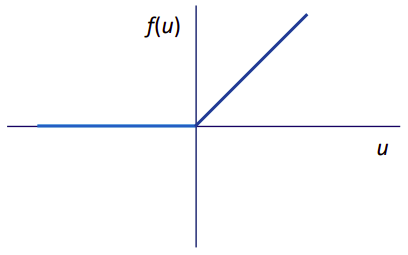
\includegraphics[width=0.5\textwidth]{images/ReLU.png} % replace with your image file name
  \caption{Γραφική μορφή συνάρτησης ReLU}
  \label{figure 14}
\end{figure} 

Αφού παρουσιάσαμε την συνάρηση ράμπας ώς συνάρτηση ενεργοποίησης, αξίζει να δούμε και μια πιο σύγχρονη παραλλαγή της, την Gaussian Error Linear Unit (GELU). Η αυξημένη πολυπλοκότητα των βαθιών μη γραμμικών μοντέλων τα καθιστά ικανά να προσαρμόζονται υπερβολικά καλά στα δεδομένα, οδηγώντας σε υπερπροσαρμογή. Αυτό συχνά απαιτεί απο τους σχεδιαστές των μοντέλων να επιλέξουν επιπλέον τεχνικές κανονικοποίησης, όπως η εισαγωγή θορύβου στα στρώματα και η απενεργοποίηση νευρώνων (Dropout). Αυτές οι τεχνικές δρούν συμπληρωματικά ώς πρός τις συναρτήσεις ενεργοποίησης και μπορούν να βελτιώσουν την ικανότητα γενίκευσης του μοντέλου. Η συνάρτηση GELU έχει σχεδιαστεί για να ενσωματώνει αυτήν τη στοχαστική συμπεριφορά πιο φυσικά, προσφέροντας μια πιο πιθανοκρατική ερμηνεία της εξόδου ενός νευρώνα. Στην πράξη, έχει δείξει ίση ή και καλύτερη απόδοση από την ReLU σε συγκεκριμένες εργασίες της όρασης υπολογιστών, της επεξεργασίας φυσικής γλώσσας και της αναγνώρισης ομιλίας. Η συνάρτηση GeLU συνδυάζει χαρακτηριστικά της απενεργοποίησης νευρώνων, της συνάρτησης ράμπας και του zoneout. Το zoneout αποτελεί τεχνική κανονικοποίησης που στοχαστικά κρατά κάποιες τιμές εξόδου των νευρώνων ίδιες με το προηγούμενο πέρασμα. Η όλη ιδέα υλοποιείται πολλαπλασιάζοντας την είσοδο του νευρώνα με 0 ή 1, όπου η επιλογή μεταξύ 0 και 1 γίνεται στοχαστικά και εξαρτάται από την τιμή της εισόδου. Συγκεκριμένα πολλαπλασιάζουμε την τιμή της εισόδου u με την κατανομή m \(\sim \mathrm{Bernoulli}\bigl(\Phi(u)\bigr)\), όπου \(\Phi(u) = P(X \leq u), \; X \sim \mathcal{N}(0, 1)\). Η κατανομή αυτή επιλέχθηκε επειδή οι τιμές των εισόδων των νευρώνων τείνουν να ακολουθούν κανονική κατανομή. Στο πλαίσιο αυτό, όσο μικραίνει η τιμή της εισόδου, τόσο πιο πιθανό είναι να μηδενιστεί. Η διαδικασία είναι τυχαία, αλλά εξαρτάται από την ίδια την τιμή της εισόδου. Η τεχνική αυτή ουσιαστικά αυτό που κάνει μηδενίζει ή αφήνει την είσοδο ίδια. Η συνάρτηση GeLU δίνεται απο την σχέση \\

\begin{equation}
\mathrm{f}(u) = u P(X \leq u) = u \Phi(u) = u \cdot \frac{1}{2} \left[1 + \operatorname{erf}\left(\frac{u}{\sqrt{2}}\right)\right].
\end{equation}\\

\noindent, όπου \(X \sim \mathcal{N}(0, 1)\) και erf(\(\cdot\)) η συνάρτηση σφάλματος, η οποία δίνεται απο την σχέση\\

\begin{equation}
\operatorname{erf}(z) = \frac{2}{\sqrt{\pi}} \int_{0}^{z} e^{-t^2} \, dt
\end{equation}\\

\noindent Η συνάρτηση GeLU μπορεί να προσεγγιστεί μέσω της σχέσης \\

\begin{equation}
f(u) \approx 0.5u \left(1 + \tanh\left[\sqrt{\frac{2}{\pi}} \left(u + 0.044715u^3\right)\right]\right)
\end{equation}\\

\noindent ή μέσω της \\

\begin{equation}
f(u) \approx u \sigma(1.702u)
\end{equation} \\

\noindent ,όπου σ(\(\cdot\)) η σιγμοειδής συνάρτηση. Η προσεγγιστικές μορφές της GeLU χρησιμοποιούνται σε περίπτωση όπου η ταχύτερος υπολογισμός της αξίζει το κόστος της ακρίβειας~\cite{hendrycks2023gaussianerrorlinearunits}. Η γραφική μορφή της συνάρτησης αυτής δίνετε παρακάτω.\\


\begin{figure}[h!]
  \centering
  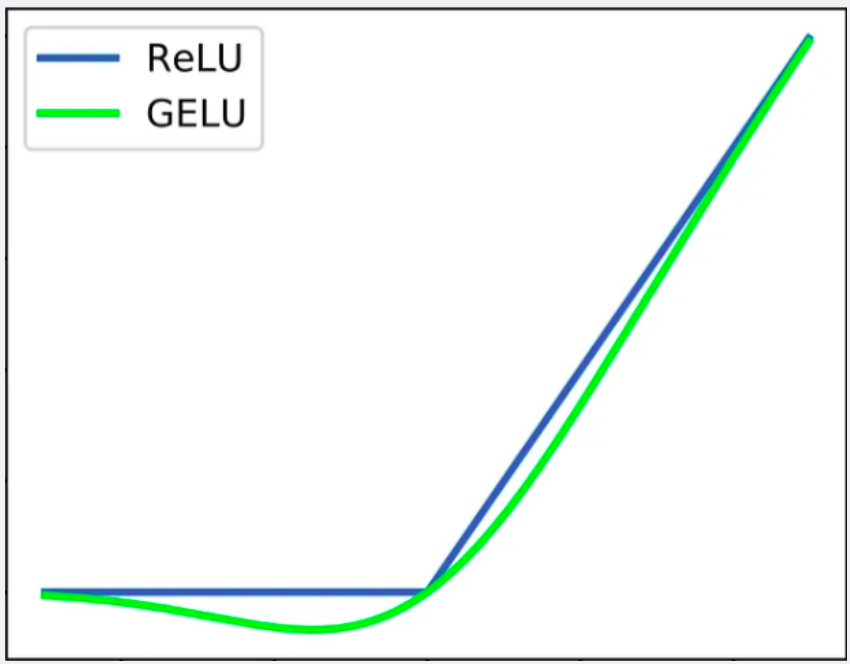
\includegraphics[width=0.5\textwidth]{images/GeLU.png} % replace with your image file name
  \caption{Γραφική μορφή συνάρτησης GeLU}
  \label{figure 14}
\end{figure}


\paragraph{Γραμμική συνάρτηση (Linear function)\\[0.5cm]}

Η γραμμική ή διαφορετικά ταυτοτική (Identity) συνάρτηση έχει πεδίο ορισμού και σύνολο τιμών το \(\mathbb{R}\). Δίνεται απο την σχέση \\

\begin{equation}
f(u) = u
\end{equation}

Παρά την απλότητά της, παρουσιάζει σημαντικά μειονεκτήματα. Η χρήση γραμμικής συνάρτησης ως συνάρτησης ενεργοποίησης περιορίζει το μοντέλο, καθώς λόγω της γραμμικής μορφής του δεν μπορεί να μάθει πολύπλοκες μη γραμμικές σχέσεις~\cite{codecademy_linear_activation_2023}. Επιπλέον, δεν είναι δυνατή η χρήση οπισθοδρόμισης για την εκπαίδευση του μοντέλου, καθώς η παράγωγος της συνάρτησης είναι σταθερή και δεν έχει σχέση με την τιμή της εισόδου u~\cite{baheti_activation_functions_2021}. Η γραφική μορφή της γραμμικής συνάρτησης δίνετε παρακάτω \\

\begin{figure}[h!]
  \centering
  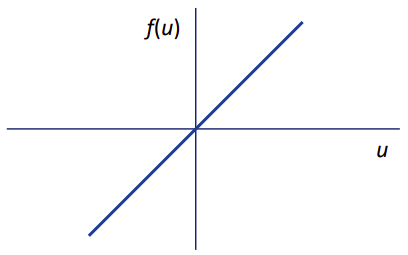
\includegraphics[width=0.5\textwidth]{images/Linear.png} % replace with your image file name
  \caption{Γραφική μορφή γραμμικής συνάρτησης}
  \label{figure 15}
\end{figure}

Η ειδική περίπτωση τεχνητού νευρώνα με συνάρτηση ενεργοποίησης την βηματική συνάρτηση καλείτε δίκτυο Perceptron~\cite{rosenblatt1958perceptron}. Το δίκτυο Perceptron είναι το πιο απλό νευρωνικό δίκτυο που μπορεί να σχεδιαστεί. 

\subsection{Νευρωνικά δίκτυα πολλών στρωμάτων}

\subsubsection{Το δίκτυο MLP}

Στα γραμμικά μοντέλα όπως το δίκτυο Perceptron οι δυνατότητες αναπαράστασης διαχωριστικών επιφανειών είναι περιορισμένες, επειδή το δίκτυο μπορεί να αναπαραστήσει μόνο επίπεδες επιφάνειες. Με άλλα λόγια το υπερεπίπεδο u=0, χωρίζει τον χώρο \(\mathbb{R}^n\) σε 2 μέρη, όπου στο ένα ισχύει f(u) = 1 και στο άλλο f(u) = 0 (Στην περίπτωση που χρησιμοποιούμε την 0/1 βηματική συνάρτηση αντί την -1/1). Η κατάσταση που προκύπτει μπορεί να οπτικοποιηθεί καλύτερα στις 2 διαστάσεις. Στον χώρο \(\mathbb{R}^2\) η εξίσωση u=\(w_1x_1 + w_2x_2 + b\) = 0 ορίζει μια ευθεία κάθετη στο διάνυσμα των συναπτικών βαρών \(\bar{w} = [w_1, w_2]^T\). Η ευθεία αυτή χωρίζει το επίπεδο σε 2 τμήματα. 

\begin{itemize}
  \item Το τμήμα πρός την κατεύθυνση του \(\bar{w}\) περιέχει τα \(\bar{x}\) για τα οποία ισχύει u > 0 (και άρα f(u) = 1)
  \item Το τμήμα πρός την αντίθετη κατέυθυνση του \(\bar{w}\) περιέχει τα σημεία \(\bar{x}\) για τα οποία ισχύει u < 0 (και άρα f(u) = 0)
\end{itemize} 

Η απόσταση της ευθείας απο την αρχή των αξόνων εξαρτάται απο την τιμή της πόλωσης \(w_0\) = b. Η σχηματική μορφή της παραπάνω ευθείας στον χώρο \(\mathbb{R}^2\) δίνεται παρακάτω.\\

\begin{figure}[h!]
  \centering
  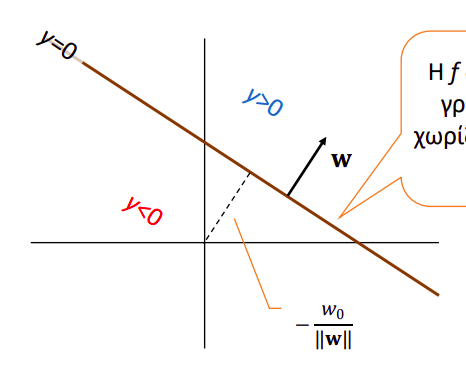
\includegraphics[width=0.5\textwidth]{images/2classclassification.png} % replace with your image file name
  \caption{Ταξινόμηση στον \(\mathbb{R}^2\) χρήση δικτύου Perceptron}
  \label{figure 16}
\end{figure}



Ο περιορισμός αυτός αίρεται με τη χρήση περισσότερων νευρώνων. Η χρήση περισσότερων κρυφών νευρώνων, θα μπορούσε να ορίσει περισσότερες διαχωριστικές ευθείες. Ο συνδυασμός των ευθειών αυτών μπορεί να μας δώσει μεγάλη ποικιλία περιοχών που θα μπορούσαμε να διαχωρίσουμε στην έξοδο. Υπάρχουν άπειρα παραδείγματα τέτοιων σχηματισμών, τα οποία μπορούν να απεικονιστούν σε διαφορετικές διαστάσεις. Στη συνέχεια παρουσιάζεται μια ενδεικτική σχηματική απεικόνιση της μορφής που μπορεί να προκύψει στον χώρο \(\mathbb{R}^2\). \\

\begin{figure}[h!]
  \centering
  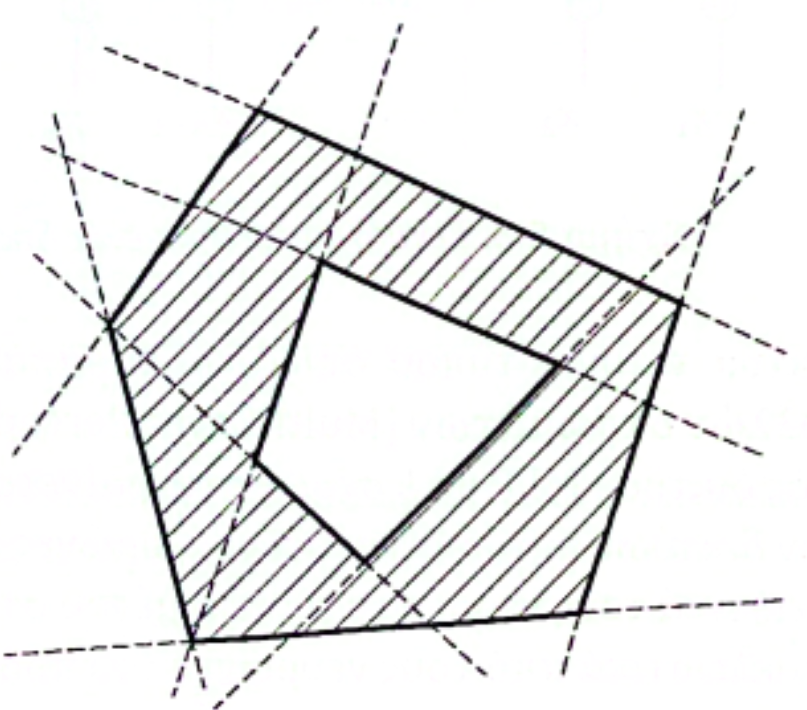
\includegraphics[width=0.5\textwidth]{images/MLP_class.png} % replace with your image file name
  \caption{Ταξινόμηση στον \(\mathbb{R}^2\) χρήση MLP}
  \label{figure 16}
\end{figure}

Δίκτυα τέτοιoυ τύπου καλούνται δίκτυα Perceptron πολλών στρωμάτων (Multi-Layer Perceptron - MLP). Η γενική αρχιτεκτονική ενός δικτύου MLP με L στρώματα φαίνετε παρακάτω. Το χαρακτηριστικό των δικτύων αυτών είναι πως οι νευρώνες του στρώματος l τροφοδοτούν αποκλειστικά τους νευρώνες του επόμενου στρώματος l+1 και τροφοδοτούνται αποκλειστικά από τους νευρώνες του προηφούμενου στρώματος l-1. \\

\begin{figure}[h!]
  \centering
  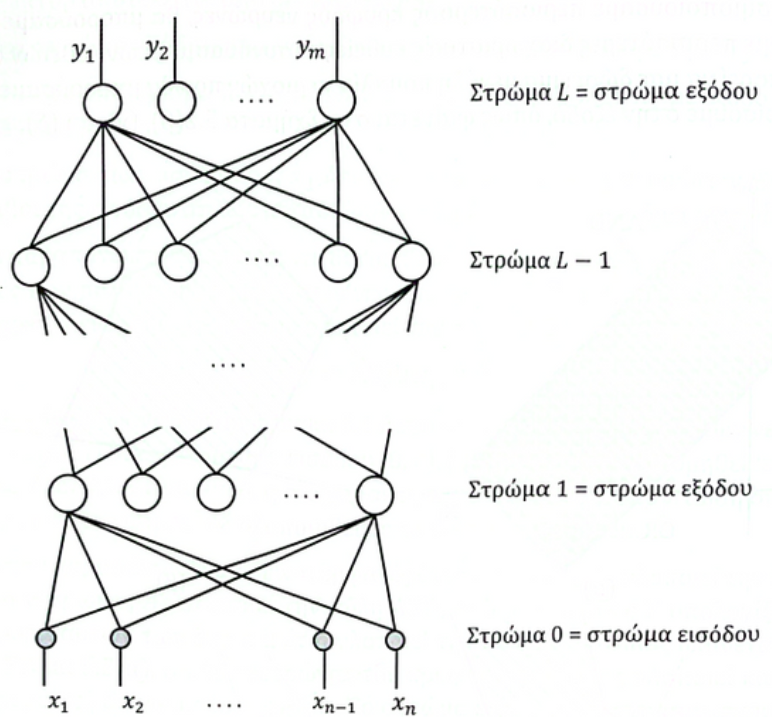
\includegraphics[width=0.7\textwidth]{images/MLP.png} % replace with your image file name
  \caption{Γενική σχηματική μορφή δικτύου Perceptron πολλών στρωμάτων}
  \label{figure 17}
\end{figure}

Τα δίκτυα Perceptron πολλών στρωμάτων στα οποία οι νευρώνες χρησιμοποιούν την βηματική συνάρτηση 0/1 ή -1/1, όπως έχουμε ήδη διαπιστώσει μπορούν να υλοποιήσουν συναρτήσεις που δεν είναι εφικτό να υλοποιηθούν με ένα απλό δίκτυο Perceptron. Ωστόσο, η χρήση της βηματικής συνάρτησης δεν προτιμάται. Ο λόγος είναι ότι οι περισσότεροι κανόνες εκπαίδευσης βασίζονται σε μεθόδους βελτιστοποίησης, οι οποίες χρησιμοποιούν παραγώγους, ενώ η βηματική συνάρτηση δεν είναι παραγωγίσιμη. Αυτή είναι μια τεχνική δυσκολία η οποία παρ'όλα αυτά ξεπερνιέται με την χρήση της σιγμοειδούς συνάρτησης. Η σιγμοειδής συνάρτηση είναι παραγωγίσιμη και μοιάζει πολύ με την βηματική συνάρτηση 0/1. \\

Εναλλακτικά μπορούν να χρησιμοποιηθούν συναρτήσεις όπως η υπερβολική εφαπτομένη, η οποία είναι παραγωγίσιμη και μοιάζει με την βηματική -1/1, η συνάρτηση ράμπας κ.ο.κ. \\

Πολύ σημαντικό είναι να αναφέρουμε πως ένα δίκτυο MLP μπορεί να υλοποιήσει οποιαδήποτε διαχωριστική επιφάνεια σε n διαστάσεις, σε αντίθεση με το απλό δίκτυο Perceptron που μπορεί να υλοποιήσει μόνο ευθείες επιφάνειες. Η απόδειξη δίνεται στο ~\cite{HORNIK1989359}. Πράγματι, άν θέλουμε να προσεγγίσουμε οποιαδήποτε διαχωριστική επιφάνεια στον χώρο \(\mathbb{R}^n\) χρησιμοποιώντας ένα MLP, αρκεί να βρούμε μια συνάρτηση g(x) τέτοια ώστε για κάποιο κατώφλι θ, ο χώρος \(\mathbb{R}^n\) να χωρίζεται σε δύο τμήματα. Για τα μισά θα ισχύει g(x) > θ και για τα άλλα μισά g(x) < θ. \\

\paragraph{Ανάκληση} είναι η διαδικασία υπολογισμού των τιμών όλων των νευρώνων του δικτύου με δεδομένες τις τιμές των εισόδων. Ορίζουμε αρχικά ως

\begin{itemize}
  \item L το πλήθος των στρωμάτων του δικτύου εκτός του στρώματος εισόδου.
  \item N(l) είναι το πλήθος των νευρώνων του στρώματος l, l = 0,...,L.
  \item \(\alpha_i(l)\) είναι οι ενεργοποιήσεις των νευρώνων του στρώματος l.
  \item \(w_{ij}(l)\) είναι το συναπτικό βάρος που συνδέει τον νευρώνα \(\alpha_j(l-1)\) του στρώματος l-1 με τον νευρώνα \(\alpha_i(l)\) του στρώματος l.
   \item \(w_{i0}(l)\) είναι η πόλωση του νευρώνα \(alpha_i(l)\) του στρώματος l.
   \item \(x_i\) = \(\alpha_i(0)\) είναι οι είσοδοι του δικτύου.
   \item \(y_i\) = \(\alpha_i(L)\) είναι οι έξοδοι του δικτύου.
\end{itemize}  

Οι ενεργοποιήσεις των νευρώνων για οποιαδήποτε στρώμα δίνονται από την σχέση\\

\begin{equation}
a_i(l) = f\left( \sum_{j=1}^{N(l-1)} w_{ij}(l) \, a_j(l-1) + w_{i0}(l) \right)
\end{equation} \\

Αυτός είναι ο τύπος ενεργοποίησης ενός νευρώνα. Όπως δείχνει η παραπάνω σχέση, ο νευρώνας i του στρώματος l δέχεται ως εισόδους τις ενεργοποιήσεις \(\alpha_i(l-1)\) των νευρώνων απο το στρώμα l-1 και ως πόλωση την τιμή \(w_{i0}(l)\). Κατά την ανάκληση μας δίνονται οι τιμές \(x_i\) των εισόδων του δικτύου, οπότε με βάση της εισόδους υπολογίζουμε πρώτα τις ενεργοποιήσεις των νευρώνων του στρώματος 1, κατόπιν βάση αυτές υπολογίζουμε τις ενεργοποιήσεις του στρώματος 2 κ.ο.κ. 

\subsubsection{Ο αλγόριθμος εκπαίδευσης Back-Propagation}

Η εκπαίδευση ενός δικτύου πολλών στρωμάτων είναι η διαδικασία καθορισμού των συναπτικών βαρών του έτσι ώστε να ικανοποιείται κάποιο κριτήριο καταλληλότητας. Αυτός είναι και ο λόγος της εκπαίδευσης σε οποιοδήποτε νευρωνικό δίκτυο. Κυριότερος εκπρόσωπος των αλγορίθμων εκπαίδευσης Peceptron πολλών στρωμάτων είναι ο αλγόριθμος Back-Propagation. Ο αλγόριθμος Back-Propagation προτάθηκε από τον Paul Werbos στη δεκαετία του 1970 στα πλαίσια της ανάλυσης μοντέλων οικονομικής και πολιτικής πρόβλεψης. Στη δεκαετία του 1980 έγινε αντιληπτό πως η μέθοδος μπορούσε να μεταφερθεί αυτούσια στην εκπαίδευση νευρωνικών δικτύων πολλών στρωμάτων και έκτοτε έγινε η πιο γνωστή και η πιο διαδεδομένη μέθοδος για τον σκοπό αυτό. \\

Βασικό χαρακτηριστικό της μεθόδου είναι η ύπαρξη στόχων. Συνεπώς, το μοντέλο ανήκει στην κατηγορία των δικτύων που εκπαιδεύονται με επίβλεψη. Έστω δίκτυο με L στρώματα, n εισόδους και m εξόδους. Ορίζουμε ως \\

\begin{itemize}
    \item $\mathbf{x}^{(p)} = \begin{bmatrix} x_1^{(p)}, \ldots, x_n^{(p)} \end{bmatrix}^T \quad \text{το p\text{-}οστό διάνυσμα εισόδου}$
    \item $\mathbf{y}^{(p)} = \begin{bmatrix} y_1^{(p)}, \ldots, y_m^{(p)} \end{bmatrix}^T \quad \text{το p\text{-}οστό διάνυσμα εξόδου}$
    \item $\mathbf{t}^{(p)} = \begin{bmatrix} t_1^{(p)}, \ldots, t_m^{(p)} \end{bmatrix}^T \quad \text{το p\text{-}οστό διάνυσμα στόχων}$
\end{itemize}

\noindent Τα δεδομένα που απαιτούνται για να εκπαιδευτεί το δίκτυο είναι τα ζεύγη διανυσμάτων $\{\mathbf{x}^{(i)}, \mathbf{t}^{(i)}\}$, i = 1,...,P. Θα ήταν ιδανικό να πετυχέναμε τάυτιση εξόδων και στόχων για κάθε πρότυπο εισόδου, ωστόσο αυτό μπορεί να μην είναι απολύτως εφικτό. Για αυτό τον λόγο επιζητούμε τη βέλτιστη προσέγγιση της επιθυμητής κατάστασης χρησιμοποιώντας ένα κριτήριο κόστους. 

\newpage

\renewcommand{\refname}{Βιβλιογραφική αναφορά}
\bibliographystyle{ieeetr}  % or another style like plain, alpha, apalike
\bibliography{references}



 

\end{document}
